% concatenated from main.tex
\documentclass[a4paper, reqno, 14pt]{amsart}

% Essential packages
\usepackage[usenames,dvipsnames]{color}
\usepackage{amsthm,amsfonts,amssymb,amsmath,amsxtra}
\usepackage[all]{xy}
\SelectTips{cm}{}
\usepackage{xr-hyper}
\usepackage[colorlinks=true, allcolors=blue]{hyperref}
\usepackage{verbatim}
\usepackage{enumerate}
\usepackage{cleveref}

% Page layout and fonts
\usepackage[margin=1.25in]{geometry}
\usepackage{mathrsfs}
\usepackage{float}
% \usepackage{showkeys}
% \usepackage{refcheck}  % optional
\usepackage{tikz}
\usetikzlibrary{positioning}

% Colors
\definecolor{myred}{rgb}{0.8,0,0}
\definecolor{myblue}{rgb}{0,0,0.8}
\definecolor{mygreen}{rgb}{0,0.6,0}

% Draw a hexagon at (x,y) with radius r, fill color, and optionally connect children recursively
\newcommand{\drawHexFractal}[4]{%
    % #1: x, #2: y, #3: radius, #4: recursion depth
    \begin{scope}[shift={({#1},{#2})}]
        % Draw filled hexagon with vertex up (rotated by 30 deg)
        \fill[gray!60] (30:{#3}) \foreach \a in {90,150,210,270,330,30} { -- (\a:{#3}) };
        % Draw colored edges (also rotated by 30 deg)
        \foreach \i/\col in {0/myred,1/mygreen,2/myblue,3/myred,4/mygreen,5/myblue} {
            \pgfmathsetmacro{\a}{30+60*\i}
            \pgfmathsetmacro{\b}{30+60*(\i+1)}
            \draw[line width=1pt,\col] (\a:{#3}) -- (\b:{#3});
        }
        % Draw vertices (but NOT the center!)
        \foreach \i in {0,...,5} {
            \pgfmathsetmacro{\a}{30+60*\i}
            \fill[black] (\a:{#3}) circle (1.3pt);
        }
        % Recursive children at vertices (not edge midpoints)
        \ifnum#4>0
            \foreach \i in {0,...,5} {
                \pgfmathsetmacro{\angle}{30+60*\i}
                \pgfmathsetmacro{\cx}{2*#3*cos(\angle)}
                \pgfmathsetmacro{\cy}{2*#3*sin(\angle)}
                % Draw green edge only from vertex to child center!
                \draw[mygreen,thick] (\angle:{#3}) -- (\cx,\cy);
                % Draw the child hexagon at (\cx,\cy) with radius 0.45*#3 (no recursion)
                % Draw a line at each corner except the one that connects to the parent
                \begin{scope}[shift={(\cx,\cy)}]
                    \pgfmathsetmacro{\r}{0.45*#3}
                    % The corner that connects to the parent is at angle = 30+60*k, which is 30+60*i
                    \pgfmathsetmacro{\parentCorner}{mod(\angle+180,360)}
                    \foreach \j in {0,...,5} {
                        \pgfmathsetmacro{\theta}{30+60*\j}
                        % If this corner is NOT the parent-connecting corner, draw the segment
                        \ifdim\theta pt=\parentCorner pt\relax\else
                            \draw[thick,black] (\theta:\r) -- ++(\theta:{0.5*\r});
                        \fi
                    }
                \end{scope}
                % Recursive call
                \drawHexFractal{\cx}{\cy}{0.45*#3}{\numexpr#4-1\relax}
            }
        \fi
    \end{scope}
}


% Extra programming and layout tools
\RequirePackage{xspace}
\RequirePackage{etoolbox}
\RequirePackage{varwidth}
\RequirePackage{enumitem}
\RequirePackage{tensor}
\RequirePackage{mathtools}
\RequirePackage{longtable}
\RequirePackage{multirow}

% Depth of Table of Contents
\setcounter{tocdepth}{1}

% Redefine symbols
\def\d{\delta}
\def\i{{^{-1}}}
\def\subset{\subseteq}
\def\supset{\supseteq}
\def\NN{\mathbb{N}}
\def\co{\mathcal{O}}
\def\ch{\mathcal{H}}
\renewcommand{\int}{\operatorname{int}}

% Declare operators
\DeclareMathOperator{\supp}{supp}
\DeclareMathOperator{\Ad}{Ad}
\DeclareMathOperator{\Ker}{Ker}
\DeclareMathOperator{\End}{End}
\DeclareMathOperator{\Span}{span}
\DeclareMathOperator{\Lie}{Lie}
\DeclareMathOperator{\Rep}{Rep}
\DeclareMathOperator{\Mod}{Mod}
\DeclareMathOperator{\Irr}{Irr}
\DeclareMathOperator{\cl}{cl}
\DeclareMathOperator{\Ch}{Ch}
\DeclareMathOperator{\Cay}{Cay}
\DeclareMathOperator{\Stab}{Stab}
\DeclareMathOperator{\Aut}{Aut}
\DeclareMathOperator{\id}{id}
\DeclareMathOperator{\fin}{fin}

% Theorem environments
\newtheorem{thm}{Theorem}[section] 
\newtheorem{prop}[thm]{Proposition}
\newtheorem{lem}[thm]{Lemma}
\newtheorem*{conj}{Conjecture}
\newtheorem{cor}[thm]{Corollary}
\newtheorem{namedthm}{Theorem}
\newenvironment{thmA}[1]{%
  \renewcommand\thenamedthm{#1}%
  \begin{namedthm}
}{%
  \end{namedthm}
}

\theoremstyle{definition}
\newtheorem{exerc}[thm]{Exercise}
\newtheorem{defn}[thm]{Definition}
\newtheorem{example}[thm]{Example}
\newtheorem*{ass}{Assumption}

\theoremstyle{remark}
\newtheorem{obs}[thm]{Observation}
\newtheorem*{rmk}{Remark}
\newtheorem*{claim*}{Claim}

% Numbering
\numberwithin{equation}{section}
\numberwithin{thm}{section}

\usepackage{enumitem}
\setlist[enumerate,1]{label=(\roman*), ref=\roman*}

% Function restriction notation
\newcommand\restr[2]{\left.\kern-\nulldelimiterspace #1 \vphantom{\big|} \right|_{#2}}

% Title info
\title{Centralizers in Hecke Algebras of Any Coxeter Group}
\author{Haiyu Chen}
% \date{}

\begin{document}
\maketitle
\begin{abstract}
We study the centralizer of a parabolic subalgebra in the Hecke algebra associated with an arbitrary (possibly infinite) Coxeter group. While the center and cocenter have been extensively studied in the finite and affine cases, much less is known in the indefinite setting. We describe a basis for the centralizer, generalizing known results about the center. Our approach combines algebraic techniques with geometric tools from the Davis complex, a CAT($0$)-space associated to the Coxeter group. As part of the construction, we classify finite partial conjugacy classes in infinite Coxeter groups and define a variant of the class polynomial adapted to the centralizer.
\end{abstract}




\section{Introduction}
\subsection{Background and Motivation}
Hecke algebras naturally arise in representation theory and play a central role in understanding the representations of finite groups of Lie type and $p$-adic groups. This paper studies a general version of Hecke algebras associated with arbitrary Coxeter groups.

Let $(W,S)$ be a Coxeter system with finite generating set $S$ and length function $\ell$. Let $R$ be a commutative ring. Suppose we are given a family of parameters $(a_s, b_s)_{s \in S}$ in $R$ such that if $s$ and $t$ are conjugate in $W$, then $(a_s, b_s) = (a_t, b_t)$. The \emph{generic Hecke algebra} $\mathcal{H} = \ch(W, S, (a_s, b_s)_{s \in S})$ is defined as the free $R$-module with basis $\{T_w\}_{w \in W}$ and multiplication rules
\[
\begin{aligned}
T_v T_w &= T_{vw} && \text{if } \ell(vw) = \ell(v) + \ell(w), \\
T_s^2 &= a_s T_s + b_s && \text{for all } s \in S.
\end{aligned}
\]
A notable special case is the Iwahori-Hecke algebra, obtained by setting $a_s = q - 1$ and $b_s = q$ for all $s \in S$ and a prime power $q$. Throughout, we assume all $b_s$ are invertible in $R$.

A guiding philosophy in representation theory is that ``characters tell everything.'' In analogy with group algebras, the character table of a Hecke algebra governs its irreducible representations. Structural subgroups such as the center and cocenter play pivotal roles: the center $Z(\mathcal{H})$ controls the number of irreducible representations, while the cocenter $\mathcal{H}/[\mathcal{H},\mathcal{H}]$ governs the space of trace functions. 

To generalize the notion of the center, we consider the centralizer of a parabolic subalgebra. Given $J \subseteq S$, let $\ch_J:=\mathcal{H}(W_J,J,(a_s,b_s)_{s\in J})$ be the subalgebra of $\ch$ generated by $\{T_s\}_{s \in J}$. The \emph{centralizer} of $\ch_J$ in $\ch$ is defined as
\[
\mathcal{Z}_{\ch}(\ch_J) := \{ h \in \ch \mid h x = x h \text{ for all } x \in \ch_J \}.
\]
When $J = S$, this recovers the center $Z(\mathcal{H})$. 

A comparison between the center and cocenter across different sizes of Coxeter groups reveals deep structural trends. In the finite case, they are both of rank $\sharp\cl(W)$ by \cite{geck2000characters}. For the affine case, the center has a basis indexed by dominant weights $P^+$ \cite{lusztig1989affine}, which are in bijection with the conjugacy classes of translations. It is further in bijection with the set of finite conjugacy classes in $W$. The cocenter \cite{he2014minimal} is indexed by all conjugacy classes $\cl(W)$. In the infinite non-affine case, the center is trivial \cite{marquis2024centre}, and the cocenter is conjectured as below. 
\begin{table}[H]
\centering
\begin{tabular}{|l|c|c|}
\hline
\textbf{Dimension} & \textbf{Center} & \textbf{Cocenter} \\
\hline
Finite Case & $\sharp \cl(W)$ & $\sharp \cl(W)$ \\
\hline
Affine Case & $\sharp P^+ = \sharp \cl^{\mathrm{fin}}(W)$\footnotemark & $\sharp \cl(W)$ \\
\hline
Infinite Non-Affine Case & Trivial & $\sharp \cl(W)$\textbf{\textcolor{red}{??}} \\
\hline
\end{tabular}
\caption{Center and cocenter comparison across different Coxeter group types}
\end{table}

This comparison indicates that when the group $W$ is larger, the center shrinks and the cocenter expands.  This work and \cite{partialcocenterADLV} on the following generalization reinforce this observation:

\begin{table}[h]
\centering
\begin{tabular}{|l|c|c|}
\hline
\textbf{Dimension} & \textbf{$\mathcal{Z}_{\mathcal{H}}(\mathcal{H}_J)$} & \textbf{$\mathcal{H}/[\mathcal{H}, \mathcal{H}_J]$} \\
\hline
General Coxeter Groups & $\sharp \cl_J^{\mathrm{fin}}(W)$ (\cref{thm:mainthmcentralizer}) & $\sharp \cl_J(W)$ (\cite{partialcocenterADLV}) \\
\hline
\end{tabular}
\caption{Comparison of partial centralizers and cocenters}
\end{table}

\subsection{Problem Setup and Main Results}

Let $\ch$ and $\ch_J$ be as above. The structure of $\mathcal{Z}_{\mathcal{H}}(\mathcal{H}_J)$ is investigated in three main steps, each centered around a key result:

\subsubsection*{Step 1: Classification of Finite $W_J$-Conjugacy Classes}

We first determine exactly which elements $w \in W$ have finite $W_J$-conjugacy classes. This is formalized in the following theorem, which may be of independent interest.

\begin{thmA}{A}[Classification of Finite $W_J$-Conjugacy Classes]
Suppose $(W,S)$ is an infinite Coxeter group and $J$ is irreducible. Then $\co_J(w)$ is finite only in the following cases:
\begin{enumerate}
    \item $J$ is spherical, i.e., $W_J$ is finite;
    \item $w \in W_{J^\perp}$;
    \item $J$ is affine, and $w = w_1 w_2$, $w_1 \in W_{J^\perp}$, $w_2 \in W_J$, and $w_2$ is a translation in $W_J$.
\end{enumerate}
Here, $J^\perp = \{ s \in S \setminus J \mid sj = js \text{ for all } j \in J \}$.
\end{thmA}

\subsubsection*{Step 2: Maximal Length Elements and Geometric Finiteness}

Two important concepts for analyzing Coxeter group conjugacy classes are cyclic shift and strong conjugation.

Roughly speaking, a cyclic shift on $w \in W$ means moving a generator from the start of a reduced expression of $w$ to the end or vice versa. We denotes $w \xrightarrow{s} w'$ if $w'=s w s$ and $\ell(w') \le \ell(w)$, $s \in S$, and denote $w \rightarrow w'$ for a sequence of such arrows.

Strong conjugation means moving the first few generators of a reduced expression of $w$ to the end while preserving the length, or vice versa. We denote strong conjugation by $w \sim w'$ when $\ell(w)=\ell(w')$ and there exists $x \in W$ such that $w'=x w x^{-1}$ and $\ell(x w)=\ell(x)+\ell(w)$ or $\ell(w x^{-1})=\ell(x)+\ell(w)$. 

A fundamental theorem for Coxeter groups states that every element can be cyclically shifted to minimal length in its conjugacy class, and any two minimal length elements are strongly conjugate \cite{marquis2018cyclically}. In this work, we develop the maximal version of this result:

\begin{thmA}{B}[Maximal Length Representatives]
Let $(W,S)$ be a Coxeter system. Let $\co_{J}$ be a $W_J$-conjugacy class of $W$. Then the following assertions hold:
    \begin{enumerate}
         \item If $\co_{J}$ is finite, then for each $u \in \co_{J}$, there exists a finite chain $u_k\xrightarrow{s_k}\cdots\xrightarrow{s_1}u$, where $u_k \in \co^{\max}_J$ and all $s_j \in J$.
         \item If $\co_{J}$ is infinite, then for each $u \in \co_{J}$, there exists an infinite chain of distinct elements $\cdots\xrightarrow{s_2}u_1\xrightarrow{s_1}u$, where all $s_j \in J$.
         \item For any $u, u' \in \co^{\max}_{J}$, we have $u \backsim_{J} u'$. (definition in \ref{defmaxequ})
    \end{enumerate}
\end{thmA}

One important step in dealing with infinite conjugacy classes is using metric geometry. We study the set
\[
U^+_J(w) := \{ w' \in W \mid w' \to_J w \}
\]
and show that it is finite if and only if $\co_J(w)$ is finite. This is achieved by applying tools from geometric group theory via the Davis complex.

The Coxeter complex $\Sigma$, constructed from cosets $\{wW_T\}$ and simplicial inclusions, encodes much of the algebraic structure of $W$. However, it is not locally finite when $W$ is infinite, preventing properly discontinuous group actions. Davis \cite{davis1994buildings} introduced a metric realization of $\Sigma$ into a complete CAT(0) space, called the \emph{Davis complex} $X$. This space is piecewise Euclidean, contractible, and admits a proper, cocompact action of $W$ by isometries. Convexity properties of displacement functions on $X$—a consequence of the CAT(0) geometry—are essential to our proof that $U^+_J(w)$ and $\co_J(w)$ have matching finiteness behavior.

\subsubsection*{Step 3: Construction of Centralizer Basis}

If $\co_J(w)$ is infinite, then the entire conjugacy class contributes nothing to the centralizer. Otherwise, we inductively define \( f^{\max}_{w,\mathcal{O}_J}\in R \), a variant of the class polynomials of Geck-Pfeiffer \cite{geck1993irreducible}, and construct a basis element for each finite $W_J$-conjugacy class.

\begin{thmA}{C}[Basis of the Centralizer]
The centralizer $\mathcal{Z}_{\mathcal{H}}(\mathcal{H}_J)$ is a free $R$-module. An $R$-basis is given by
\[
\left\{ z_{\mathcal{O}_J} = \sum_{w \in W} b_w^{-1} f^{\max}_{w, \mathcal{O}_J} T_{w^{-1}} \right\}_{\mathcal{O}_J},
\]
where the index $\mathcal{O}_J$ ranges over all \textbf{finite} $W_J$-conjugacy classes in $W$. Each sum is finite.
\end{thmA}

\subsubsection*{Conjecture on the Cocenter}

Motivated by our work, we propose the following conjecture, consistent with known results in the finite and affine settings \cite{geck1993irreducible, he2014minimal}, and a partial result is known in \cref{prop:cocenterbasis}:

\begin{conj}
The cocenter $\mathcal{H}/[\mathcal{H}, \mathcal{H}]$ has a basis indexed by the set of conjugacy classes $\cl(W)$.
\end{conj}




\subsection{Acknowledgement}
I am deeply grateful to Xuhua He for suggesting this problem and for his invaluable guidance throughout the project. I also thank Michael McBreen for his consistent support during my Ph.D. studies. I am sincerely thankful to Felix Schremmer for the insightful discussions and helpful suggestions.
























\section{Preliminaries}

    Let $(W,S)$ be a Coxeter system with $S$ a finite set. The Coxeter group $W$ is equipped with the length function $\ell: W \to \NN$ and the Bruhat order $\le$. 
    
    The subgroups $W_J:=\langle J\rangle\subseteq W$ ($J\subseteq S$) are called \emph{standard parabolic subgroups} of $W$, and their conjugates are \emph{parabolic subgroups} of $W$. For $w\in W$, each $W_J$-coset $W_Jw$ contains a unique minimal length element $\min W_J w$. Let $^J W=\{\min W_J w\ |\ w\in W\}$. Moreover, $\ell( yx)=\ell(y)+\ell(x)$ for any $x\in {}^JW$, $y \in W_J$. The above notions can be similarly defined for $W^J$. For $K,K'\subset S$, we denote ${}^{K'}W^K:={}^{K'}W\cap W^K$.
    
        We say $J\subset S$ \emph{spherical} if $W_J$ is finite; otherwise we say $J$ is non-spherical. The reason is that a building is spherical if and only if its Weyl group is a finite Coxeter group. See, for example, \cite{abramenko2008buildings}. We say $J$ is \emph{affine} if $W_J$ is affine. We say $J$ (resp. $W_J$) is \emph{irreducible} if it does not decompose nontrivially as a disjoint union $J=J_1\sqcup J_2$ with $s_1s_2=s_2s_1$ for all $s_1\in J_1$ and $s_2\in J_2$. Denote $J^{\perp}:=\{s\in S\setminus J \ | \ st=ts \ \forall t\in J\}$. For $w\in W$, let $w\cdot J:=w J w \i$.

\subsection{Partial Cyclic Shift Classes}
    In 1993, Geck-Pfeiffer \cite{geck1993irreducible} pointed out that two special kinds of conjugation action are important in the study of Hecke algebras, namely cyclic shift and strong conjugation.
    Let $J\subset S$ be a subset.
    \begin{defn}
    
    \begin{enumerate}
        \item For $w, w' \in W$, we write $w \xrightarrow{s} w'$ if $w'=s w s$ and $\ell(w') \le \ell(w)$, $s \in S$; We write $w \xrightarrow{J} w'$ if there exists a sequence $w=w_0, w_1, \cdots, w_n=w'$ of elements in $W$ such that for any $k$, $w_{k-1} \xrightarrow{s} w_k$ for some $s \in J$.  We write $w \approx_{J} w'$ if $w \xrightarrow{J} w'$ and $w' \xrightarrow{J} w$, equivalently, $w \xrightarrow{J} w'$ and $\ell(w)=\ell(w')$.
        
        
        \item We call $w, w' \in W$ \emph{elementarily strongly $J$-conjugate} if $\ell(w)=\ell(w')$ and there exists $x \in W_J$ such that $w'=x w x^{-1}$ and $\ell(x w)=\ell(x)+\ell(w)$ or $\ell(w x^{-1})=\ell(x)+\ell(w)$. We call $w, w'$ {\it strongly $J$-conjugate} if there is a sequence $w=w_0, w_1, \cdots, w_n=w'$ such that for each $i$, $w_{i-1}$ is elementarily strongly $J$-conjugate to $w_i$. We write $w \sim_{J} w'$ if $w$ and $w'$ are strongly $J$-conjugate.

    \end{enumerate}  
    \end{defn}
    \begin{rmk}
    \begin{enumerate}
        \item In all notation above, we omit $J$ if $J=S$;
        \item Note that $\approx_J$ implies $\sim_J$.
    \end{enumerate}
        Both $\approx_{J}$ and $\sim_{J}$ are equivalence relations. The equivalence classes under $\approx_{J}$ are called the \emph{$J$-cyclic shift classes}. 
        
    \end{rmk}

    





% It is obvious that $\approx_J$ implies $\sim_J$.

% By the calculation in Hecke algebra, it is easy to see that the coefficient of $x=\sum_{x\in W} x_wT_w\in \mathcal{Z}_{\ch}(\ch_{J})$ should satisfy the following relation
% \begin{itemize}
%     \item If $w\sim_J w'$ then $x_w=x_w'$;
%     \item If $w\xrightarrow{s} w'$ and $\ell(w)>\ell(w')$, $s\in J$, then $x_{w'}=b_sx_w-a_sx_{sw}$.
% \end{itemize}

\begin{defn} We set
    $U^+_J(w):=\{w'\in W \ | \ w'\xrightarrow{J} w\}.$
\end{defn}
Note that $U^+_J(w)\subset W_J\cdot w$.

An important result for the calculation is the following. Here we only review the classical result for the case of finite Coxeter groups and $J=S$. 

\begin{thm}[\cite{geck1993irreducible}]\label{thm:minimal_thm_finite}
    Let $(W,S)$ be a finite Coxeter group. Let $\co^{\min}$ be the set of minimal length elements in $\co$. Then
    \begin{enumerate}
        \item For any $w\in W$, $w\rightarrow w'$ for some $w'\in\co^{\min}$.
        \item For any two $w,w'\in\co^{\min}$, $w\sim w'$.
    \end{enumerate}
\end{thm}
It is later generalized to extended affine Weyl groups \cite{he2014minimal} and we will review this result for general Coxeter groups later (see \cref{thm:mingeneral}).

\subsection{Davis complex}
Basics on Davis complexes can be found in \cite{davis1994buildings,davis2008geometry} and also in \cite{marquis2020structure}.
\subsubsection{Coxeter complex}
A Coxeter complex $\Sigma=\Sigma(W,S)$ is a simplicial complex with simplices being the cosets $\{wW_I\ |\ w\in W,I\subsetneq S \}$, with face relation being opposite to the usual set inclusion $\subset$. The maximal simplices $wW_\emptyset=\{w\}$ are called \emph{chambers}. Denote by $\Ch(\Sigma)$ the set of chambers. The \emph{fundamental chamber} $C_0$ is the chamber corresponding $\{e\}$. Chambers are in bijection with elements in $W$. We sometimes use elements in $W$ to represent a chamber.

Any two \emph{adjacent} chambers are of the form $\{w\}$ and $\{ws\}$, where $w\in W, s\in S$, contains a \emph{panel} $m_s$ of type $s$, which is the 1-codimensional intersection of the chambers. In this case, we say they are \emph{$s$-adjacent}. A gallery $\Gamma=(D_0,D_1,\dots,D_k)$ of length $k$ is a sequence of chambers such that $D_{i-1}$ and $D_i$ are $s_i$-adjacent. We say $(s_1,s_2,\dots,s_k)$ is the \emph{type} of $\Gamma$. If $s_i\in J\subset S$ for all $i$, then we call $\Gamma$ to be a \emph{$J$-gallery}.

For any two chambers $C,D\in \Ch(\Sigma)$, the galleries from $C$ to $D$ are called \emph{minimal} if their lengths are minimal among all galleries from $C$ to $D$. We define the chamber distance $d_{\Ch}(C,D)$ to be the length of the minimal galleries between $C$ and $D$. For $C=vC_0$, $D=wC_0$, we have $d_{\Ch}(C,D)=\ell(v\i w)$. Now fix $w\in W$. Chambers in Coxeter complex encodes information on conjugates of $w$ through the following function $\pi_w:\Ch(\Sigma)\to W$, $v C_0\mapsto v\i wv$. For $D\in \Ch(\Sigma)$, the chamber distance $d_{\Ch}(D,wD)=\ell(\pi_w(D))$.

The group $W$ acts on $\Sigma$ by left multiplications, which are simplicial isometries of $\Sigma$. Elements of $s\in S$ act by \emph{simple reflections}, and their conjugates are \emph{reflections}. Each reflection $r=r_m$ has a fixed-point set $m$ called a \emph{wall}.  

We may visualize $\Sigma$ as a simplicial complex with the fundamental domain being a simplex of dimension $|S|-1$. It is identified with the fundamental chamber described above. Each coset $wW_I$ is a simplex of codimension $|I|$ (or dimension $|S|-|I|-1$).  For each $w\in W$ we attach a copy of the fundamental chamber and glue them by face relations. We may also draw a Cayley graph $\Cay(W,S)$ on $\Sigma$ as follows. A vertex $\{v\}$ is the barycenter $x_D$ of the chamber $D=vC_0$. An $s$-edge is drawn between $x_C$ and $x_D$ for $C,D\in \Ch(\Sigma)$ that are $s$-adjacent. 

Every wall divides $\Sigma$ into two \emph{half-spaces}: the graph $\Cay(W,S)\setminus m$ has two connected components whose vertex sets are the barycenters of chambers in these half-spaces. Walls can be visualized as 1-codimensional hyperplanes in the simplicial complex. Every panel is contained in a unique wall $m$: The $s$-adjacent chambers $wC_0$ and $wsC_0$ contain a panel $m_s$, which is contained in a wall $m$ corresponding to reflection $r_m=wsw\i$. We say the wall $m$ \emph{separates} chambers $C,D\in \Ch(\Sigma)$ if they are in different half-spaces associated with $m$. We also say the $|S|$ walls $\{m\ |\ r_m=wsw\i,\ s\in S\}$ are walls of $wC_0$. The chamber distance $d_{\Ch}(C,D)$ equals the number of walls separating $C$ and $D$. 

We may read off cosets $wW_J$ from $\Sigma$ by the notion of a $J$-residue. For a chamber $D=wC_0$, the set of chambers $R_J(D)$ connected to $D$ by a $J$-gallery is called a \emph{$J$-residue} of $D$. We see that $R_J(wC_0)$ corresponds to elements in $wW_J$. Its stabilizer in $W$ is $\Stab_W(R_J(wC_0))=wW_Jw\i$. A wall $m$ separates two chambers of a residue $R$ if and only if $r_m\in \Stab_W(R)$, in which case we call it a \emph{wall of $R$}.



\subsubsection{Davis complex}
The Davis complex $X=X(W,S)$ is a metric realization of Coxeter complex $\Sigma(W,S)$. It is a complete CAT($0$) cellular complex with piecewise Euclidean metric $d$, with a natural action of $W$ by cellular isometries. While the fundamental domain of a Coxeter complex is a simplicial complex of dimension $|S|-1$, that of a Davis complex is usually not. We now describe a cellular construction of the Davis complex as follows. 

Let $I\subset S$ be a \emph{spherical} subset, meaning the parabolic group $W_I$ is finite. The $|I|$-dimensional cell $P_I$ is called a Coxeter cell, defined as follows. $W_I$ acts on an $I$-dimensional Euclidean space $V_I$ with simple reflections $s\in I$ acting by linear reflections. The wall $m_s$ is a hyperplane fixed by $s$. The collection of walls $(m_s)_{s\in I}$ delimit a simplicial cone $C_I$ in $V_I$. Let $x_I$ be the point in the interior of $C_I$ with distance $1$ to each wall $m_s$. Then $P_I$ is the convex hull of points $W_Ix_I$, with induced Euclidean metric from $V_I$. Note that if $I\subset J$ are both spherical, then $P_I$ is a face of $P_J$.

The $1$-skeleton $X^{(1)}$ is the Cayley graph of $(W,S)$. For each $I\subset S$ spherical, we glue $I$-dimensional cells $P_I$ to the Cayley subgraph of $(W_I,I)$ inductively from low to top dimensions according to face relations above. The metric $d$ is obtained by gluing each Euclidean metric on $P_I$, for $I\subset S$ spherical. Since $W$ acts on the Cayley graph preserving spherical residues, it induces an action on $X$ by cellular isometries.

The chamber system of Coxeter complexes can also be realized in Davis complexes. We realize chambers of $\Sigma$ inside $X$ as a closed convex subset. For $C=vC_0$, and let $x_C:=\{v\}$ be a vertex in $X^{(1)}$. For each spherical residue $wR_I$, $I\subset S\text{ spherical}$ containing $C$ corresponds to a polytope $P_I$ in $X$ with $x_C=x_I$. Define $C:=\bigcup_{I\subset S\text{ spherical}} P_I\cap C_I$. We refer to $x_C$ as the \emph{barycenter} of $C$. We identify chambers and walls of $\Sigma$ with their realization of $X$. We also set $\Ch(X)=\Ch(\Sigma)$ to be the collection of chambers in $X$. 



\begin{example}
The Davis complex of the Coxeter group
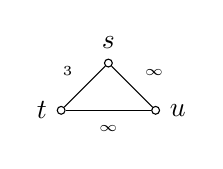
\begin{tikzpicture}[scale=0.6,baseline={(current bounding box.center)}]
  \node[circle, draw, inner sep=1pt, label=above:$s$] (s) at (0,1) {};
  \node[circle, draw, inner sep=1pt, label=left:$t$] (t) at (-1,0) {};
  \node[circle, draw, inner sep=1pt, label=right:$u$] (u) at (1,0) {};
  \draw (s) -- (t) node[midway, above left=0.5pt and 1pt] {\tiny 3};
  \draw (s) -- (u) node[midway, above right=0.5pt and 1pt] {\tiny $\infty$};
  \draw (t) -- (u) node[midway, below=2pt] {\tiny $\infty$};
\end{tikzpicture}
has the fundamental chamber
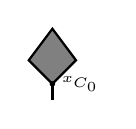
\begin{tikzpicture}[baseline={(current bounding box.center)}]
  \coordinate (top) at (0,0.4);
  \coordinate (right) at (0.3,0);
  \coordinate (bottom) at (0,-0.3);
  \coordinate (left) at (-0.3,0);
  \coordinate (c0) at (0,-0.3);
  \filldraw[fill=black!50, thick] (top) -- (right) -- (bottom) -- (left) -- cycle;
  \fill (c0) circle (1pt);
  \node[right] at (c0) {\tiny $x_{C_0}$};
  \draw[thick] (c0) -- ++(0,-0.2);
\end{tikzpicture},
which is shaded in the picture below.
It is given by $C=\bigcup_{I\subset S\text{ spherical}} P_I\cap C_I$. The hexagon in the picture is $P_{\{s,t\}}$. The three lines are walls of three generators. The Davis complex is shown below.

\medskip

\noindent
\begin{figure}[h]
    \centering
    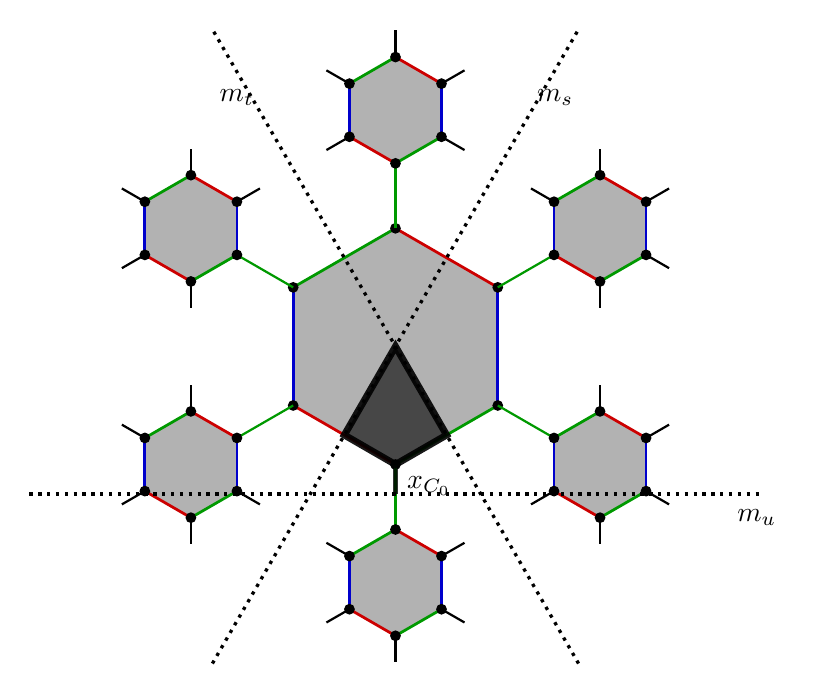
\begin{tikzpicture}[scale=1.5]
        \drawHexFractal{0}{0}{1}{1}
        \draw[dotted,very thick] ({-3.1*cos(60)}, {-3.1*sin(60)}) -- ({3.1*cos(60)}, {3.1*sin(60)});
        \draw[dotted,very thick] ({-3.1*cos(120)}, {-3.1*sin(120)}) -- ({3.1*cos(120)}, {3.1*sin(120)});
        \draw[dotted,very thick] (-3.1,-1.25) -- (3.1,-1.25);
        \node at ({2.3*cos(60)}, {2.3*sin(60)}) [above right=-2pt] {$m_s$};
        \node at ({2.3*cos(120)}, {2.3*sin(120)}) [above left=-2pt] {$m_t$};
        \node at (0, -1.25) [below right=2pt and 120pt] {$m_u$};
        \node at (0, -1) [below right=1pt] {$x_{C_0}$};
        \fill[black, opacity=0.6]
            (0, 0)
            -- (0.433, -0.75)
            -- (0, -1)
            -- (-0.433, -0.75)
            -- cycle;
        \draw[line width=2.5pt, black, opacity=0.9]
            (0, 0)
            -- (0.433, -0.75)
            -- (0, -1)
            -- (-0.433, -0.75)
            -- cycle;
        \draw[black, line width=2pt, opacity=0.8]
            (0, -1) -- (0, -1.25);
    
        
    \end{tikzpicture}
    \caption{Davis complex of the Coxeter group ($3,\infty,\infty$).}
\end{figure}

\end{example}













\subsection{Class Polynomials}
Class polynomials arise from studying the cocenter $\ch/[\ch,\ch]$. The theory of conjugacy classes of finite Coxeter groups can be found in \cite[\S 8]{geck2000characters}. We will summarize some important results for a finite Coxeter group $(W,S)$ here.

\begin{lem}\label{lem:sameimg}
    If $w\sim w'$, then $T_w\equiv T_{w'} \mod [\ch,\ch]$.
\end{lem}
\begin{proof}
    Write $w'=xwx\i$ with $\ell(w)=\ell(w')$ and $x\in W_J$. We have either $\ell(xw)=\ell(w)+\ell(x)$ or $\ell(wx\i)=\ell(w)+\ell(x)$. As we assume $\{b_s\}_{s\in S}$ are invertible, $T_x$ is invertible. In the first case, $T_{w'}=T_x T_w T_{x}\i$. Hence $T_w-T_{w'}= T_w-T_x T_w T_{x}\i=(T_wT_x-T_xT_w)T_x\i\in [\ch,\ch]$. The second case is similar.
\end{proof}

        Let $\cl(W)$ be the set of all conjugacy classes in $W$. For each finite conjugacy class $\co$, we choose once and for all $w_{\co}\in \co^{\min}$ a representative of minimal length.

        By \cref{thm:minimal_thm_finite}, every element can be cyclically reduced to minimal length. 
        When \( w \xrightarrow{s} w' \), we have
        \[
        T_w \equiv 
        \begin{cases}
        T_{w'} & \text{if } \ell(w) = \ell(w'), \\
        b_s T_{w'} + a_s T_{sw} & \text{if } \ell(w) > \ell(w')
        \end{cases}
        \mod [\mathcal{H}, \mathcal{H}].
        \]
        
        Indeed for the second case, write \( w' = sws \), we compute
        \[
        T_s T_w = T_s(b_s T_{sws} + a_s T_{sw}) = b_s T_{ws} + a_s T_w = T_w T_s.
        \]
        Hence, by \cref{thm:minimal_thm_finite}, we may inductively, express $T_w$ into linear combination of $T_{w_\co}$. The coefficients $f_{w,\co}\in R$ are called the \emph{class polynomials}. The class polynomials $f_{w,\co}$ satisfy the following properties. If $w$ is a minimal length element, then $f_{w,\co}=\delta_{\{w\in \co\}}$. For smaller length $w$, by \cref{thm:minimal_thm_finite}, $f_{w,\co}$ can be calculated inductively:
        \begin{equation} \label{eq:fmin-recursion}
            f_{w',\co}
              = \begin{cases}
                  f_{w,\co}, & \text{if } w \approx w', \\[6pt]
                  b_s\,f_{w,\co} \;+\; a_s\,f_{s w,\co}, & \text{if } w' \xrightarrow{s} w\text{ and } \ell(w')>\ell(w), s\in S.
                \end{cases}
        \end{equation}
        
        \begin{prop}\cite[Theorem 8.2.3]{geck2000characters}
            For each $w\in W$, we have
            \begin{equation}
                T_w\equiv \sum_{\co\in \cl(W)} f_{w,\co} T_{w_{\co}} \mod [\ch,\ch].
            \end{equation}
            Moreover, the class polynomials $f_{w,\co}$ are uniquely determined by this equation.
        \end{prop}
    \begin{rmk}
        By this proposition, the uniqueness of the class polynomial is equivalent to the linear independence of the basis elements (the image of) $\{T_{w_\co}\}_{\co}$ in the cocenter $\ch/[\ch,\ch]$.
    \end{rmk}




\section{Classification of finite partial conjugacy classes}
    Let $w\in W, J\subset S$. In this section, we classify when the $W_J$-conjugacy classes in $W$ are finite. 
    
    % This is clearly the case when $W_J$ is finite or when $w\in W_{J^\perp}$. We want to make the following assumption.
    % \begin{ass}
    %     Assume $J\subset S$ to be irreducible and non-spherical. Also we assume $w\notin W_{J^\perp}$.
    % \end{ass}
    
     Denote by $\bar{w}\in {}^JW^J$ the unique minimal length element in $W_JwW_J$. 
     
     Denote $w\cdot J:=w J w \i$.
     
     Following \cite[Corollary 2.3,2.6]{he2007minimal}, setting $K_v=\max\{K \subset J\mid  v\cdot K=K\}$ and define the \textit{partial conjugation} of $W_J$ acting on $W$ by $x\cdot y=xyx^{-1}$. For an automorphism $\sigma: W\to W$, we may define the \textit{twisted conjugation} by $x\cdot_\sigma y=xy\sigma(x)\i$.
    
    
    Moreover, we have the following correspondence on the $\Ad(v)$-twisted conjugacy classes $\mathcal{C}$ in $W_{K_v}$ and the $W_J$-conjugacy classes in $W_J\cdot (vW_{K_v})$.


    \begin{prop} \label{thm:partialconjdecom}
    Let $J\subset S$.
    \begin{enumerate}
        \item We have $$W=\sqcup_{v \in  {}^JW} W_J \cdot (v W_{K_v}).$$ 
        
    
        \item For each $v\in {}^JW$, write $K=K_v$ and consider an automorphism
        $\sigma: W_K\to W_K$, $\sigma(x)=vxv\i$. For an $\sigma$-twisted conjugacy class $\mathcal{C}$ in $W_K$, we have $$W_J\cdot v\mathcal{C}=W_J \times^{W_K} v\mathcal{C}$$ 
    where the right-hand side is the quotient space given by $(w_J,vx)\sim (w_Jw_K\i,w_Kvxw_K\i)$, for $w_J\in W_J$, $x\in \mathcal{C},w_K\in W_K$. 
    \end{enumerate}
    \end{prop}

    \begin{proof}
        \begin{enumerate}
            \item This is \cite[Corollary 2.6]{he2007minimal}.
            \item Note that $\sigma=\Ad(v)$, and $xv=v\sigma\i(x)$ for any $x\in W_K$. 

            On the one hand, write $w_J=w_1w_K, w_1\in W_J^K$, $w_K\in W_K$. Then for $x\in \mathcal{C}$, $w_J\cdot vx=w_1w_Kvxw_K\i w_1\i=w_1\cdot v\sigma\i(w_K)xw_K\i\in w_1\cdot v\mathcal{C}$.

            On the other hand, assume $w_J\cdot vx=vx'$, for $w_J\in W_J,x,x'\in \mathcal{C}$. Then $w_J=vx'x\i v\i\in vW_Kv\i \subset W_K$. Moreover, $w_J\cdot vx=v\sigma\i(w_J)xw_J\i$. Hence, $x'=\sigma\i(w_J)xw_J\i\in \mathcal{C}$ and $w_J\in W_K$.
        \end{enumerate}
    \end{proof}

    \begin{cor} \label{cor:counting}
        In the setting above, $$\sharp W_J\cdot v\mathcal{C}=\sharp W_J /W_K\times \sharp\mathcal{C}$$ 
    \end{cor}

    We quote two results to be used in our proof.
    \begin{lem}\cite[Lemma 3.3]{marquis2024centre}\label{lem:MarquisComb}
        Let $w\in W$. If there exists a non-spherical subset $J\subset S$ so that $H:=J\cap \bar{w}\cdot J$ is spherical, then $U^+_J(w)$ is infinite.
    \end{lem}
    The proof is purely combinatorial.
    \begin{lem}\cite[Lemma 2.1]{capraceMarquis2013open}\label{lem:normalizer}
        Let $J\subset S$ be a subset so that all irreducible components are non-spherical. Then the normalizer $N_W(W_J)=W_J\times W_{J^\perp}=W_{J\sqcup J^\perp}$.
    \end{lem}
    The proof is root-theoretic.
    
    \begin{thm}\label{thm:classification} Suppose $(W,S)$ is an infinite Coxeter group and $J$ is irreducible. Then $\co_J(w)$ is finite only in the following cases. 
    \begin{enumerate}
        \item $J$ is spherical, i.e., $W_J$ is finite;
        \item $w\in W_{J^\perp}$;
        \item $J$ is affine, and $w=w_1 w_2$, $w_1\in W_{J^\perp}$, $w_2\in W_J$, and $w_2$ is a translation in $W_J$.
        
    \end{enumerate}
    Here, $J^\perp=\{s\in S\setminus J\ | \  sj=js\text{ for all } \ j\in J \}.$
    \end{thm}
    \begin{proof}
        In all three cases, it is clear $\co_J(w)$ is finite. Only case (iii) needs some illustration. In fact, if we consider the decomposition of an affine Weyl group $W_J=W_0\ltimes X$ into a finite Weyl group $W_0$ and the coroot lattice $X$, and write $\tilde{w}=wt^\mu, \tilde{w}\in W_J, w\in W_0, \mu\in X$ (written exponentially as $t^\mu$), we have $wt^\mu w^{-1} =t^{w\mu}$ and $t^{\mu'}t^\mu t^{-\mu'}=t^\mu$. Hence $(wt^\mu) w't^{\mu'} (wt^\mu)\i = ww'w\i t^{w(w'\i\mu-\mu+\mu')}$ and the infinitude of conjugacy class of $w't^{\mu'}$ only depends on $\{w'\i\mu-\mu\ |\ \mu\in X\}$. It is finite only for translation elements ($w'=e$).
        
        Conversely, we want to show that these are the only three cases that can occur. Suppose $\co_J(w)$ is finite. The first two cases are obvious, so we may assume $J\subset S$ to be irreducible and non-spherical, and $w\notin W_{J^\perp}$, and we want to reduce it to the case $(iii)$.

        First, we claim that all proper subsets of $J$ are spherical. Assume not, then we may find a minimal non-spherical subset $J'\subsetneq J$ so that all proper subsets of $J'$ are spherical. Moreover, $J'\sqcup J'^\perp\subsetneq J$ as $J$ is irreducible. We may conjugate $w$ inside $U_J^+(w)$ so that $\supp w=J$, otherwise, for any $s\in J\setminus \supp w$, either $\ell(sws)=\ell(w)+2$ or $s\in (\supp w)^\perp$ (see e.g. \cite[Lemma 2.37]{abramenko2008buildings}). But then this implies $w\notin N_W(W_{J'})=W_{J'\sqcup J'^\perp}$ by \cref{lem:normalizer}. Hence $\bar{w}\cdot J'\neq J'$ (otherwise $w$ will normalize $W_{J'}$). As a result, $H:=J'\cap \bar{w}\cdot J'\subsetneq J'$ is spherical. Then $U^+_{J'}(w)$ is infinite by \cref{lem:MarquisComb} and so does $U^+_J(w)$ and $\co_J(w)$.

        Next, we have $\bar{w}\cdot J= J$, for otherwise, $\bar{w}\cdot J\cap J$ would be spherical and by \cref{lem:MarquisComb}, $\co_J$ would be infinite. Let $v\in {}^JW$ so that $w\in W_J\cdot vW_{K_v}$ in \cref{thm:partialconjdecom}(i). By \cref{cor:counting},  $\sharp W_J /W_K$ being finite forces $K_v=J$, i.e., $v\cdot J=J$. Hence, $v\in N_W(W_J)=W_J \times W_{J^\perp}$. As $v\in {}^JW$, we have $v\in W_{J^\perp}$. In this case, $\Ad(v)=\id$, and up to $W_J$ conjugation, $w=vw_J$ for some $w_J\in W_J$. Therefore, the partial conjugacy class $\sharp \co_J(w)=\sharp \co_J(w_J)$ is finite if and only if $J$ is affine and $w_J$ is a translation \cite[lemma 4.6]{marquis2024centre}.
        \end{proof}

    \section{Infinitude of cyclic shift classes}
        In this section, we will show that the cyclic shift class is infinite precisely when the conjugacy class is infinite, generalizing results in \cite[Section 4]{marquis2024centre}.
        
        Let $X=X(W,S)$ be a Davis complex associated with the Coxeter group $(W,S)$ with metric $d$. Let $J\subset S$. Let $X_J$ be the subcomplex of $X$ with the $1$-skeleton being the Cayley graph of $W_J$ and only Coxeter cells $P_I$, $I\subset J$ spherical. Note that as the metric is piecewisely defined on each $P_J$, it makes sense to restrict the metric on each $P_J$, and they glue into a metric, denoted as $d_J$, on $X_J$, making $(X_J,d_J)$ into a Davis complex, which is again a CAT($0$)-space. Note that although $d_J$ is different from $\restr{d}{X_J}$ in general, if for $x,y\in X$, the geodesic $[x,y]\subset X_J$, then $d_{J,w}=d_w$ on $[x,y]$. For $w\in W$, define the three important functions 
        $$d_w:X\to \mathbb{R}, x\mapsto d(x,wx)$$
        $$d_{J,w}:X_J\to \mathbb{R}, x\mapsto d_J(x,wx)$$ $$d_{\Ch,w}:\Ch(X)\to \mathbb{N}, C\mapsto d_{\Ch}(C,wC)$$
        Note that when $J=S$, $d_{J,w}=d_w$. We will use the same notation $d_{\Ch}$ for the chamber distance of any Davis complex when the context is clear. We shall explain the basic properties of these three functions.
        The first two are displacement functions on Davis complexes. It is a result of CAT($0$)-space that displacement functions are convex, see for example \cite[II, 6.2(3)]{bridson2013metric}. In particular, both $\restr{d_w}{X_J}$ and $d_{J,w}$ are convex on $X_J$. The third function is a chamber-wise function related to the lengths of conjugates of $w$: for $D\in \Ch(X)$, $d_{\Ch,w}(D)=d_{\Ch}(D,wD)=\ell(\pi_w(D))$. In particular, the statement that two $s$-adjacent chambers $D$ and $D'$, with $d_{\Ch,w}(D)\leq d_{\Ch,w}(D')$ translates to $\pi_w(D')\xrightarrow{s} \pi_w(D)$. 

        We call a chamber $C\in \Ch(X)$ as \emph{$(w,J)$-local maximum} if every non-decreasing $J$-gallery is flat, i.e., for every $\Gamma=(D_0=C,D_1,\dots,D_k)$ in $\Ch(X)$, with $d_{\Ch,w}(D_i)\leq d_{\Ch,w}(D_{i+1})$ for all $i$, we have $d_{\Ch,w}(D_i)= d_{\Ch,w}(D_{i+1})$ for all $i$. 

    First, we quote a result on the relations of $d_{\Ch,w}$ and $d_w$.

    \begin{prop}\cite[Proposition 4.4]{marquis2024centre}\label{prop:chamber_to_metric}
        Let $X'=X'(W',S')$ be a Davis complex with metric $d_w'$. Let $w\in W'$. Let $C,D\in \Ch(X')$ be adjacent chambers separated by wall $m$. Let $x\in \int(C)$, $y:=r_m(x)\in \int(D)$ and $z:=[x,y]\cap m$. Then $d_{\Ch,w}(C)<d_{\Ch,w}(D)$ implies $d_w'$ is strictly increasing on $[z,y]$.
    \end{prop}

    This result is essentially due to the convexity of $d_w$ and the strong convexity of $X$.

    We also need to quote a lemma for the Davis complex.
    \begin{lem}[{\cite[Lemma 2.5]{marquis2024centre}}] \label{lem:extgeod}
        Assume that $(W,S)$ is infinite, irreducible, but all proper subsets of $S$ are spherical.
        \begin{enumerate}
        \item
        Let $x$ be the barycentre of a chamber $C$, let $m_1,\dots,m_k$ be the walls of $C$, and for each $i=1,\dots,k$, choose a point $x_i\in [x,r_{m_i}(x)]\setminus \{x\}$. Then the convex hull of $\{x_1,\dots,x_k\}$ contains an open neighbourhood of $x$.
        \item 
        Every geodesic segment in $X$ can be extended to a geodesic line.
        \end{enumerate}
    \end{lem}

    \begin{prop}\label{prop:localmaximum}
        Assume that all proper subsets of $J$ are spherical. Let $w\in W$. If there exists a $(w,J)$-local maximum, all $W_J$-conjugates of $w$ are of the same length.
    \end{prop}

    \begin{proof}
        Let $C$ be a $(w,J)$-local maximum and consider the set of $(w,J)$-local maxima $C_{\approx}:=\{D\in \Ch(X)\ |\ \text{there is a $J$-gallery } (D_0=C,D_1,\dots,D_k=D) \text{ with } d_{\Ch,w}(D_i)=d_{\Ch,w}(C) \text{ for all }i\}$. Denote by $x_D$ the barycenter of the chamber $D$. 
        
        First, we claim that the set $\{d_w(x_D)\ |\ D\in C_{\approx}\}$ is finite. As $d_{\Ch,w}$ is constant on $C_{\approx}$, the set $\{\pi_w(D)\ |\ D\in C_{\approx}\}$ is finite. Moreover, $\pi_w(D)=\pi_w(D')$ if and only if $D$ and $D'$ are in the same $Z_W(w)$-orbit, so $C_{\approx}$ is covered by finitely many $Z_W(w)$-orbits of chambers. But then $d_w$ is constant on $Z_W(w)$-orbits, the set is finite as claimed.

        Now we may modify $C$ inside $C_{\approx}$ such that $d_w(x_C)$ is maximal. Let $D_i$ be the $J$-adjacent chambers of $C$ separated by walls $m_i$, $i=1,\dots,k$. By assumption of $C$, we have $d_{\Ch,w}(D_i)\leq d_{\Ch,w}(C)$. Hence we have only two cases, either $d_{\Ch,w}(D_i)<d_{\Ch,w}(C)$ or $d_{\Ch,w}(D_i)= d_{\Ch,w}(C)$. We claim that only the second case will happen. In the first case, by \cref{prop:chamber_to_metric}, $d_w$ is strictly increasing on $[x_i,x_C]$ where $x_i:=[x_{D_i},x_C]\cap m_i$. In the second case, we have $d_w(x_{D_i})\leq d_w(x_{C})$ by maximality of $x_C$. As $d_w$ is convex, either it is strictly increasing on some $[x_i,x_C]$ for some $x_i\in [x_{D_i},x]\setminus\{x\}$ or it is constant on $[x_{D_i},x_C]$ (in which case we set $x_i=x_{D_i}$). Note that as $[x_{D_i},x_C]\subset X^{(1)}\subset X_J$, we may replace $d_w$ into $d_{J,w}$. If the first case does occur, then $d_{J,w}$ is strictly increasing on some $[x_j,x_C]$. By \cref{lem:extgeod}, we may extend $[x_j,x_C]$ to $[x_j,y]$ with $[x_j,x_C]\subsetneq [x_j,y]\subset X_J$, so that $d_{J,w}(x_i)\leq d_{J,w}(x_C)<d_{J,w}(y)$ for all $i$ and $y$ lies in the convex hull of $\{x_1,\dots,x_k\}$ inside $X_J$. But then this contracts to the convexity of $d_{J,w}$ on $X_J$.

        We have shown that for any chamber $D$ that is $J$-adjacent to $C$, we have $D\in C_{\approx}$ and $d_w(x_{D_i})=d_w(x_{C})$. We may inductively conclude this is the case for all chambers on a $J$-gallery from $C$. The proof is complete. 

        
    \end{proof}

    \begin{thm}\label{thm:infU} Let $w\in W$ and $J\subset S$ irreducible. Then $\co_J(w)$ is infinite if and only if $U_J^+(w)$ is infinite.
    \end{thm}

    \begin{proof}
        The if direction is automatic. It remains to show the only if direction. Assume $\co_J(w)$ is infinite. Then $J$ must be non-spherical. 
        
        We may assume all proper subsets of $J$ are spherical, for otherwise, both $U_J^+(w)$ and $\co_J(w)$ are infinite by the argument in the proof of \cref{thm:classification}. 
        
        If $U_J^+(w)$ is finite, then the maximal length element inside $U_J^+(w)$ will produce a $(w,J)$-local maximum, which, by \cref{prop:localmaximum}, further implies $\co_J(w)$ is finite.
    \end{proof}

    \section{The centralizers $\mathcal{Z}_{\ch}(\ch_J)$}
        
        \subsection{The generic Hecke algebra}
            Let $(W,S)$ be a Coxeter group with the length function $\ell$. Let $R$ be a commutative ring. Let $\ch(W,S,(a_s,b_s)_{s\in S})$ be a \emph{generic Hecke algebra} as in the introduction.

            We may use another equivalent definition in practice, namely 
           \begin{equation*}
                T_sT_w = 
                \left\{
                \begin{aligned}
                    &a_s T_{w} + b_s T_{sw} & \text{if } \ell(sw) < \ell(w) \\
                    &T_{sw} & \text{if } \ell(sw) > \ell(w)
                \end{aligned}
                \right.
            \end{equation*}
            
            As centralizers of products are products of centralizers, we may assume $J$ is irreducible.
            \begin{ass}
                In the sequel, we assume $b_s$ are all invertible in $R$ and $J$ is irreducible.
            \end{ass} 
            As a consequence, $\{T_w\}_{w\in W}$ are all invertible. 
    
        Denote by $\ch=\ch(W,S,(a_s,b_s)_{s\in S})$ and $\ch_J=\ch(W_J,J,(a_s,b_s)_{s\in J})$ as a subalgebra of $\ch$.
        The centralizer (or \emph{partial center}) $\mathcal{Z}_{\ch}(\ch_{J})$ is a generalization of the center.

        \begin{prop}\label{prop: diamond}
            Write $x=\sum_{w\in W}x_wT_w$, $x_w\in R$. Then $x\in \mathcal{Z}_{\ch}(\ch_{J})$ if and only if
            \begin{enumerate}
                \item $x_w=x_{w'}$ whenever $w\approx_J w'$;
                \item $x_{w'}=b_sx_w-a_sx_{sw}$ whenever $w\xrightarrow{s} w'$ and $\ell(w)>\ell(w')$ for $s\in J$.
            \end{enumerate}
        \end{prop}

        \begin{proof}
            For $z\in \ch$ and $w\in W$, we use $(z)_w$ to denote the coefficient of the basis element $T_w$ in $z$, for example, $(x)_w=x_w$.

            We first show the only if part.
            \begin{enumerate}
                \item It suffices to show $x_w=x_{w'}$ for $w\xrightarrow{s} w'$ with $\ell(w')=\ell(w)$. We may assume $w'\neq w$.
                
                By the exchange property of Coxeter groups, we cannot have both $\ell(sw)<\ell(w)$ and $\ell(ws)<\ell(w)$. Indeed, $\ell(sw)<\ell(w)$ implies there must exist a reduced expression $w$ starting with $s$, say $w=s_0s_1s_2\cdots s_k$ with $s=s_0$. But then $\ell(ws)<\ell(w)$ implies $ws=s_0s_1\cdots \hat{s_j}\cdots s_k$ with $\hat{}$ denoting omission. If $j\neq 0$ then $\ell(sws)<\ell(w)$. If $j=0$, then $ws=sw$ and that further implies $w'=sws=ssw=w$.
                
                Hence either $\ell(sw)>\ell(w)=\ell(w')$ or $\ell(ws)>\ell(w)=\ell(w')$.

                In the first case, $(T_sx)_{sw}=x_w+a_sx_{sw}$ and $(xT_s)_{sw}=x_{sws}+a_sx_{sw}$. Hence $x_{w'}=x_w$. The second case is similar.

                \item In this case, we have $\ell(sws)<\ell(ws)=\ell(sw)<\ell(w)$ and $sw\approx_J ws$. Then $(T_sx)_{sw}=b_sx_w$ and $(xT_s)_{sw}=a_sx_{sw}+x_{sws}$. Hence $x_{w'}=b_sx_w-a_sx_{sw}$. 
            \end{enumerate}

            Now we show the if part, i.e., for $s\in J$, we want to show $T_sx=xT_s$ when $x_w$, $w\in W$ satisfy both conditions. For each $w\in W$, $s\in J$, there are two cases. If $|\ell(sws)-\ell(w)|=2$ or ($\ell(sws)=\ell(w)$ and $|\ell(ws)-\ell(sw)=2|$), we are in the situation of $(ii)$. By the proof in $(i)$ above, the case $\ell(w)=\ell(sws)>\ell(ws)=\ell(sw)$ is trivial. The only case left is $\ell(w)=\ell(sws)<\ell(ws)=\ell(sw)$. But then this implies $sws\approx_J w$, and $sw\approx_J ws$. We are in the situation of $(i)$. Hence $T_sx=xT_s$ for any $s\in J$.
        \end{proof}
    \begin{rmk}
        The proof does not assume $\{b_s\}_{s\in S}$ are invertible. 
    \end{rmk}
    \begin{rmk}
        Note that in (ii), we also have $x_{sw}=x_{ws}$ by (i).
    \end{rmk}
    \begin{rmk}
        It seems likely $(i)$ holds for a stronger condition for $w\sim_J w'$. Moreover, the reduction of $T_w$ inside the cocenter also follows relations similar to the class polynomials. This observed relationship can be formalized through the duality between the Hecke algebra $\ch$ and its completion $\widehat{\ch}$ (direct product of $W$-many basis elements). The partial cocenter with respect to the parabolic subalgebra $\ch_J$ inside $\ch$ is naturally dual to the centralizer $Z_{\widehat{\ch}}(\ch_J)$ of $\ch_J$ within the completion $\widehat{\ch}$. This generalizes the duality via the symmetrizing form discussed in \cite{geck1997centers}.
    \end{rmk}

    We aim to define a maximal version of the class polynomial to record the coefficients of all $T_w$ in the reduction given in \cref{prop: diamond}. For that, we need a foundation for reducing elements to their maximal lengths. 
    
    \subsection{Reduction theorem and variations}
        We want to state the reduction theorem and its variations, generalizing the result in the finite case \cite{geck1993irreducible} and the affine case \cite{he2014minimal}.

        Let $(W,S)$ be a Coxeter system. Let $\Aut(W,S)=\{\delta\in \Aut(W)\ |\ \delta(S)=S\}$. Let $\tilde{W}=W\rtimes \Aut(W,S)$. For $J\subset S$ and $\delta\in \Aut(W_J,J)$, we can define the (partial) $\delta$-twisted conjugation $x\cdot y=xy\delta(x)\i$ for $x\in W_J,y\in W$. We could also define $\delta$-twisted conjugacy class $\co_\delta$, $\delta$-cyclic shift $w\rightarrow_\delta w'$, $\delta$-strong conjugation $w\sim_\delta w'$ and their partial versions $w\rightarrow_{\delta,J} w'$, $w\sim_{\delta,J} w'$, see for example, \cite[\S 3.1]{he2007minimal}. We use the word ``untwisted'' for cases when $\delta=\id$.
        
        \begin{thm}[\cite{marquis2018cyclically, marquis2020structure}]\label{thm:mingeneral}
             Let $(W,S)$ be a Coxeter system and let $\delta\in \Aut(W,S)$. Let $\co_\delta$ be a $\delta$-twisted conjugacy class of $W$, and let $\co^{\min}_{\delta}$ be the set of minimal length elements of $\co_\delta$. Then the following assertions hold:
            \begin{enumerate}
                 \item For each $w \in \co_{\delta}$, there exists $w' \in \co^{\min}$ such that
            $w \rightarrow_{\d} w'$.
            
                \item Let $w, w' \in \co^{\min}_\delta$, then $w \sim_{\d} w'$.
            \end{enumerate}
        \end{thm}

        \begin{rmk}
            The statement in \cite{marquis2018cyclically} is proved for untwisted conjugacy classes in $W$. In $(ii)$, they use tight conjugation, which is a special type of strong conjugation. By \cite[Remark 6.9]{marquis2020structure}, the untwisted statements can be upgraded to work for $\tilde{W}$. By \cite[Remark 3.6]{marquis2020structure}, the statement can be reduced to a twisted statement in $W$ as above.
        \end{rmk}

        The above result can be made into the partial conjugation version via the following trick.
        
        \begin{cor}Let $(W,S)$ be a Coxeter system and $J\subset S$. Let $\delta\in \Aut(W_J,J)$. Let $\co_{\delta,J}$ be a $\delta$-twisted $W_J$-conjugacy class of $W$, and let $\co^{\min}_{\delta,J}$ be the set of minimal length elements of $\co_{\delta,J}$. Then the following assertions hold:
            \begin{enumerate}
                 \item For each $w \in \co_{\delta,J}$, there exists $w' \in \co_{\delta,J}^{\min}$ such that
            $w \rightarrow_{\d,J} w'$.
            
                \item Let $w, w' \in \co^{\min}_{\delta,J}$, then $w \sim_{\d,J} w'$.
            \end{enumerate}
        \end{cor}
        \begin{proof}
            Define a new Coxeter group $(\hat{W}, S\sqcup\{s_{J,\infty}\})$ with $s_{J,\infty} j=js_{J,\infty}$ for all $j\in J$ and $s_{J,\infty} s$ having infinite order for $s\in S\setminus J$. Consider the embedding $\hat{}: W\to \hat{W}$, $w\mapsto \hat{w}:=ws_{J,\infty}$. Then $\hat{w}\rightarrow_\d \hat{w'}$ in $\hat{W}$ is equivalent to $w \rightarrow_{\d,J} w'$, and $\hat{w}\sim_\d \hat{w'}$ in $\hat{W}$ is equivalent to $w \sim_{\d,J} w'$. Therefore, applying \cref{thm:mingeneral} to $\hat{W}$ will give the desired result.
        \end{proof}

    We can also have the maximal length element version of the above corollary. Before doing this, we need a variant of the relation $\sim$. (Notice the difference between $\sim$ and $\backsim$.)
    \label{defmaxequ}
    
    Let \( w, w' \in W \) be such that \( \ell(w) = \ell(w') \). We shall write \( w \overset{x}{\backsim} w' \) if \( w' = xwx\i \) for some \( x \in W_J \) and if \( \ell(xw) = \ell(w) - \ell(x) \) or \( \ell(wx\i) = \ell(w) - \ell(x) \). 
    Again, we also write \( w \backsim_J w' \) if there exist sequences of elements \( x_i\in W_J, w_i \in W \) (\( 1 \leq i \leq n \)) such that \[ w \overset{x_1}{\backsim} w_1 \overset{x_2}{\backsim} \dots \overset{x_n}{\backsim} w_n = w'. \] 


    Now we want to prove the maximal length theorem. We need two lemmas. We will use the following setting.
    
    Assume $J\subset S$ to be spherical, and $w'\in W$. Then the double closet $W_Jw'W_J$ contains a unique maximal element, denoted as $w$. Then any element $u\in W_Jw'W_J$ is of the form $u=w_1ww_2$, $w_1,w_2\in W_J$ with $\ell(u)=\ell(w)-\ell(w_1)-\ell(w_2)$. For a finite conjugacy class $\co_J$, denote the set of maximal length elements as $\co_J^{\max}$.
    \begin{lem}\label{lem:maxdoublecoset}
        Let $u=w_1ww_2\in W_JwW_J$, and $v=ww_2w_1\in wW_J$. Denote the conjugacy class of $u,v$ by $\co_J$. Then $u\in \co_J^{\max}$ if and only if $v\in \co_J^{\max}$ and $\ell(w_2w_1)=\ell(w_2)+\ell(w_1)$.

        In fact, if we write $w_1=s_1s_2\cdots s_k$, then $u\in \co_J^{\max}$ if and only if \\ $s_{t+1}\cdots s_{k-1}s_kww_2s_1s_2\cdots s_t\in \co_J^{\max}$ and is reduced for all $t$.
    \end{lem}
    \begin{proof}
        As $\ell(v)=\ell(w)-\ell(w_2w_1)$, and $\ell(w_2w_1)\leq \ell(w_2)+\ell(w_1)$. Hence $\ell(u)\leq \ell(v)$ with equality if and only if $\ell(w_2w_1)=\ell(w_2)+\ell(w_1)$. The same proof works for the in fact part.
    \end{proof}

    \begin{lem} Let $K:=\{s\in J\ |\ wsw\i\in W_J \}$. Then \label{lem:maxWK}
    \begin{enumerate}
        \item $K=\{s\in J\ |\ wsw\i\in J \}$;
        \item $W_K=\{x\in W_J\ |\ wxw\i\in W_J \}$
    \end{enumerate}
    Hence, $\d:=\Ad(w):(W_K,K)\to (W_{\d(K)},\d(K))$ is an isomorphism of Coxeter systems.
    \end{lem}
    \begin{proof}
        \begin{enumerate}
            \item Let $v=wsw\i\in W_J$. Then $\ell(vw)=\ell(ws)=\ell(w)-1$. Then $\ell(v)=1$.
            \item Follows from $(i)$ as simple reflections in $W_K$ is necessarily contained in $K$.
        \end{enumerate}
    \end{proof}

    
    \begin{cor}\label{cor:maximalthm}
    Let $(W,S)$ be a Coxeter system and $J\subset S$. Let $\co_{J}$ be a $W_J$-conjugacy class of $W$. Then the following assertions hold:
            \begin{enumerate}
                 \item If $\co_{J}$ is finite, then for each $u \in \co_{J}$, there exist a finite chain $u_k\xrightarrow{s_k}u_{k-1}\xrightarrow{\dots}u_1\xrightarrow{s_1}u$, where $u_k \in \co^{\max}_J$ and all $s_j\in J$.
                 \item If $\co_{J}$ is infinite, then for each $u \in \co_{J}$, there exist an infinite chain of distinct elements $\xrightarrow{\dots}u_2\xrightarrow{s_2}u_1\xrightarrow{s_1}u$, where all $s_j\in J$.
            
                \item For any $u, u' \in \co^{\max}_{J}$, we have $u \backsim_{J} u'$.
            \end{enumerate}
        \end{cor}

    \begin{proof}
        For infinite $\co_J$, \cref{thm:infU} implies $(ii)$.
        
        According to the classification \cref{thm:classification}, either $J\subset S$ is spherical or affine.
        Let $J$ be spherical and $u\in W$. Write $w$ for the unique longest element in $W_JuW_J$. Then $u=u_1wu_2$, for $u_1,u_2\in W_J$. We have $wu_2u_1\rightarrow_J u$ as $\ell(wu_2u_1)=\ell(w)-\ell(u_2u_1)\geq \ell(w)-\ell(u_2)-\ell(u_1)=\ell(u)$. We may thus assume $u=wy\in wW_J$. By \cref{lem:maxdoublecoset}, we may assume $u'\in\co^{\max}_J$ are of the form $u'=wy'\in wW_J\cap \co^{\max}_J$. Now for $x\in W_J$, $$wy=xwy'x\i \iff y=(w\i xw)y'w(w\i xw)\i w\i=zy'(\Ad(w)\cdot z)\i,$$
        where $z:=w\i xw$. By \cref{lem:maxWK}, $z\in W_K$ and if we define $W_K$-action on $W_J$ by $z\cdot_{\Ad(w)}y =zy(\Ad(w)\cdot z)\i$, called $\Ad(w)$-twisted conjugation, then we have $wy$ is $W_J$-conjugate to $wy'$ if and only if $y$ is $\Ad(w)$-twisted $W_K$-conjugate to $y'$. Thus, $wy'\rightarrow_J wy\iff y\rightarrow_{K,\Ad(w)} y'$. Similarly $wy'\backsim_J wy\iff y\sim_{K,\Ad(w)} y'$ by \cref{lem:maxdoublecoset}.

        Let $J\subset S$ be affine. By the proof of \cref{thm:classification}, every conjugate of a translation element is of the same length. The claim holds trivially.
    \end{proof}
    \subsection{A variation of class polynomial}
        Now we define a variation of the class polynomial $f_{w,\co_J}$ in \cite[\S 8.2]{geck2000characters}. Let $w\in W$, and $\co_J$ be a finite $W_J$-conjugacy class. According to \cref{thm:classification}, there are three cases. For $w\in W_J$, $w_1\in W_{J^\perp}$, define $f^{\max}_{ww_1,\co_J}=f^{\max}_{w,\co_J}$. If $J$ is affine, then $f^{\max}_{w,\co_J}=1$ if $w\in \co_J$ and $f^{\max}_{w,\co_J}=0$ otherwise. If $J$ is spherical, we define $f^{\max}_{w,\co_J}$ inductively as follows.
        If $w$ is a maximal length element, then $f^{\max}_{w,\co_J}=1$ for $w\in \co_J$ and $f^{\max}_{w,\co_J}=0$ otherwise.  For a smaller length $w$ we inductively define 
        \begin{equation} \label{eq:fmax-recursion}
            f^{\max}_{w',\co_J}
              = \begin{cases}
                  f^{\max}_{w,\co_J}, & \text{if } w \sim_J w', \\[6pt]
                  b_s\,f^{\max}_{w,\co_J} \;+\; a_s\,f^{\max}_{s w,\co_J}, & \text{if } w' \xrightarrow{s} w\text{ and } \ell(w')>\ell(w), s\in J.
                \end{cases}
        \end{equation}
        We set $f^{\max}_{w,\co_J}=0$ for all other cases.\\

        Note that the inductive formula for $f^{\max}_{w,\co_J}$ is the same as that for the class polynomial $f_{w,\co_J}$ in \cref{eq:fmin-recursion}, except we change $\sim$ to $\backsim$. The main difference of $f^{\max}_{w,\co_J}$ and $f_{w,\co_J}$ is the initial value. Here, we used the assumption that $b_s$ is invertible.

        Note also that $\approx_J$ implies $\backsim_J$, so in particular, $f^{\max}_{s w,\co_J}=f^{\max}_{ws,\co_J}$ in the case $w' \xrightarrow{s} w$, $\ell(w')>\ell(w)$.

        With a slight abuse of terminology, we also call $f^{\max}_{w,\co_J}$ the (max version of) \emph{class polynomial}. This polynomial shares similar properties to those in \cite[\S 8.2]{geck2000characters}.

        Apriori, the class polynomial $f^{\max}_{w,\co_J}$ depends on each $s$ used to conjugate $w$ to its maximal length. But we shall see that this would not happen. 

        
        \begin{lem}\label{lem:sameimg}
            If $w\backsim_J w'$, then $T_w\equiv T_{w'} \mod [\ch_J,\ch]$.
        \end{lem}
        \begin{proof}
            Write $w'=xwx\i$ with $\ell(w)=\ell(w')$ and $x\in W_J$. We have either $\ell(xw)=\ell(w)-\ell(x)$ or $\ell(wx\i)=\ell(w)-\ell(x)$. In the first case, $T_w=T_{x\i}T_{xw}$ and $T_{w'}=T_{w'x}T_{x\i}$. Hence $T_w-T_{w'}=T_{x\i}T_{xw}-T_{xw}T_{x\i}\in [\ch_J,\ch]$. The second case is similar.
        \end{proof}

        Let $\cl^{\fin}_J(W)$ be the set of all finite $W_J$ conjugacy classes in $W$. For each finite conjugacy class $\co_J$, we choose once and for all $w_{\co_J}\in \co^{\max}_J$ a representative of maximal length.
        \begin{lem}\label{lem:Tw_and_class_poly}
            For $w\in W$, and $J$ is spherical or affine, we have
            \begin{equation}
                T_w\equiv \sum_{\co_J\in \cl^{\fin}_J(W)} f^{\max}_{w,\co_J} T_{w_{\co_J}} \mod [\ch_J,\ch],\label{eqn:linearcomb}
            \end{equation}
            where the sum is finite.
        \end{lem}
        
        \begin{proof}
            
            First for $w, w' \in \co^{\max}_{J}$, then $T_w\equiv T_{w'} \mod [\ch_J,\ch]$ by \cref{cor:maximalthm} and \cref{lem:sameimg}.

            According to the inductive definition of $f^{\max}_{w,\co_J}$ is not zero only when it is part of some cyclic shift process. When $J$ is spherical, $f^{\max}_{w,\co_J}$ is only related to $f^{\max}_{u,\co_J}$ for $u\in W_JwW_J$ which is a finite set. When $J$ is affine, the sum is just one term. Hence, the sum above is always finite.
            
            As the affine case is trivial, it remains to prove for the spherical case. For $w$ is not of maximal length, by \cref{cor:maximalthm}, there exist $w'\approx w$ and $s\in J$ so that $\ell(sw's)> \ell(w')=\ell(w)$. By \cref{lem:sameimg}, we have $T_w\equiv T_{w'}\mod [\ch_J,\ch]$. We may treat $w$ as $w'$ and prove for the case $\ell(sws)>\ell(sw)=\ell(ws)>\ell(w)$. We claim that $$T_{sws}\equiv b_sT_{w}+ a_sT_{sw} \mod [\ch_J,\ch].$$ Indeed, $ T_sT_{sw}-T_{sw}T_s=a_sT_{sw}+b_sT_w-T_{sws} \mod [\ch_J,\ch]$. But then this is exactly the definition of $f^{\max}_{w,\co_J}$.
        \end{proof}

      
        
        \begin{prop}\cite{partialcocenterADLV}\label{prop:cocenterbasis} 
        For spherical $J$, $\mathcal{H}/[\mathcal{H}_J,\mathcal{H}]$ has a basis given by $\{T_{w_{\co_J}}\}_{\co_J\in\cl_J(W)}$.
        \end{prop}

        
        \begin{cor}
            The $f^{\max}_{w,\co_J}$ is uniquely determined by the \cref{eqn:linearcomb}.
        \end{cor}

        \begin{proof}
            For $J$ affine, every element in a finite conjugacy class is of the same length, so no reduction will occur. For $J$ spherical, by \cref{lem:Tw_and_class_poly}, the uniqueness of $f^{\max}_{w,\co_J}$ is equivalent to the linear independence of the basis given in \cref{prop:cocenterbasis}. 
        \end{proof}

        Denote $b_w=b_{s_1}b_{s_2}\cdots b_{s_k}$ for $w=s_1s_2\cdots s_k$ some/any reduced expression. This is well-defined by Matsumoto's theorem. See, for example, \cite[\S 1.2]{geck2000characters}.
        
        \begin{thm}\label{thm:mainthmcentralizer} A basis of the centralizer $\mathcal{Z}_{\mathcal{H}}(\mathcal{H}_{J})$ is given by
        $$\{z_{\mathcal{O}_J}=\sum_{w\in W} b_w^{-1} f^{max}_{w,\mathcal{O}_J} T_{w\i}\}_{\mathcal{O}_J\in \cl_J^{\fin}(W)}$$
        
        Here, each sum is a finite sum.
        \end{thm}

        \begin{proof}
            Each sum is finite as $\co_J$ is finite as $f^{max}_{w,\mathcal{O}_J}$ vanishes for almost all $w$.
            First, we check that $z_{\co_J}\in \mathcal{Z}_{\mathcal{H}}(\mathcal{H}_{J})$ as in \cref{prop: diamond}. By definition, $b_w$ stays the same for conjugacy classes of $w$, and also $f^{max}_{w,\mathcal{O}_J}$ is stable under $\approx_J$. When $sws\xrightarrow[]{s} w$ (thus $sw\i s\xrightarrow[]{s} w\i$) with $\ell(sws)>\ell(w)$, by definition of $f^{max}_{w,\mathcal{O}_J}$ at \cref{eq:fmax-recursion}, we have 
            $$b_w^{-1} f^{max}_{w,\mathcal{O}_J}T_{w\i}=b_sb_{sws}^{-1}f^{max}_{sws,\mathcal{O}_J}T_{sw\i s}-a_sb_{ws}^{-1}f^{max}_{ws,\mathcal{O}_J}T_{sw\i}.$$

            As each $w\in \co_J^{\max}$ only appears in one $z_{\co_J}$, it is obvious that $\{z_{\co_J}\}_{\co_J}$ are linearly independent. It remains to show  $\{z_{\co_J}\}_{\co_J}$ spans $\mathcal{Z}_{\mathcal{H}}(\mathcal{H}_{J})$. 

            Let $x=\sum_{w\in W}x_wT_w\in \mathcal{Z}_{\mathcal{H}}(\mathcal{H}_{J})$. Let $v$ be an element with $\ell(v)$ maximal and $x_v\neq 0$ in the expression of $x$. Then we claim that $v\in \co^{\max}_J$ in its conjugacy class $\co_J$. First, we see that $\co_J$ must be finite, for otherwise, by \cref{thm:infU}, there exist $v'\in W$ with $v'\rightarrow_{J} v$ and $\ell(v')>\ell(v)$, and \cref{prop: diamond} (ii) together with maximality of $v$ forces $x_v=0$. For the same reason, if $v\notin \co^{\max}_J$, then \cref{cor:maximalthm} implies there exist $v'\in \co^{\max}_J$ with $v'\rightarrow_{J} v$ and $\ell(v')>\ell(v)$ and this forces $x_v=0$. The claim follows. Repeat the argument for $x-b_{v\i}z_{\co_J}$, we see that $\{z_{\co_J}\}_{\co_J\in \cl^{\fin}_J(W)}$ spans $\mathcal{Z}_{\mathcal{H}}(\mathcal{H}_{J})$.
           
        \end{proof}


    \begin{rmk}
        We give another argument for spanning using Nakayama's lemma. We use a specialization argument in \cite{lusztig1983singularities}.

            We write $a_s$ as a shorthand for $\{a_s\}_{s\in S}$. Similarly for $b_s$. Consider a specialization $\ch\to \mathbb{Z}[W]$, $b_s\mapsto 1, a_s\mapsto 0$. Denote  the image of $z_{\co_J}$ under this map by $\overline{z_{\co_J}}$. Clearly $\overline{z_{\co_J}}$ spans $\mathcal{Z}_{\mathbb{Z}[W]}(\mathbb{Z}[W_{J}])$. Let $A=\mathbb{Z}[a_s,b_s,b_s\i]_{(b_s-1,a_s)}$. Then $A/(b_s-1,a_s)\cong\mathbb{Z}$. By Nakayama's lemma, $\{z_{\co_J}\}_{\co_J}$ spans  $\mathcal{Z}_{\mathcal{H}}(\mathcal{H}_{J})$ over $A$. As both $\{z_{\co_J}\}_{\co_J}, \mathcal{Z}_{\mathcal{H}}(\mathcal{H}_{J})\subset \ch$, the coefficients of $z\in \mathcal{Z}_{\mathcal{H}}(\mathcal{H}_{J})$ in  $\{z_{\co_J}\}_{\co_J}$ are necessarily in $\mathbb{Z}[a_s,b_s,b_s\i]$. The proof is complete.
    \end{rmk}
    \begin{rmk}
        One would expect similar results to work for twisted centralizers: for a Coxeter system isomorphism $\d:(W_J,J)\to(W_{J'},J')$ 
\[
\mathcal{Z}_{\ch,\d}(\ch_J) := \{ h \in \ch \mid h x = \d(x) h \text{ for all } x \in \ch_J \}.
\]
    The main difference in the proof would be the classification of finite twisted partial conjugacy classes and the basis for the twisted cocenter. This is beyond the scope of this paper.
    
    \end{rmk}




































% \section{Backups}



%    The local Langlands program predicts a connection between irreducible smooth representations of $p$-adic reductive groups $G(F)$ and the Weil-Deligne representations from the Weil-Deligne group to the dual group of $G$. This connection provides one motivation for the study of smooth representations of $p$-adic reductive groups. According to \cite{borel1976admissible,de1988homology}, the admissible representations of $G(F)$ admitting a vector fixed by an Iwahori subgroup $\mathcal{I}$ are in one-to-one correspondence with the simple modules of the Hecke algebra $\ch(G,\mathcal{I},\mathbb{C})$. Conjecturally, classifying the simple $\ch(G,\mathcal{I},\mathbb{C})$ modules, combined with the theory of types, leads to a classification of the complex irreducible representations of $G(F)$ \cite{vigneras2003modular}. Therefore, studying simple $\ch(G,\mathcal{I},\mathbb{C})$-modules fits one of the research themes in Oxford mathematics.

%     One promising approach to studying simple $\ch:=\ch(G,\mathcal{I},\mathbb{C})$-modules is through the cocenter. The cocenter is dual, by the trace map, to the (complexification of the) Grothendieck group $R(\ch)$ of finite-dimensional $\ch$-modules. This is highly related to the interest of the research group led by \textbf{Prof. Dan Ciubotaru} at the Mathematical Institute. In a paper \cite{ciubotaru2017cocenters}, Ciubotaru and He study the rigid cocenter of the $\ch$, and their results show that the quantities about the cocenters can be made independent of the parameters of the Hecke algebras. In my doctoral thesis, I study the Hecke algebra with arbitrary parameters of a general Coxeter group, with a conjecture about its cocenter. This conjecture can be regarded as a potential generalization of their result from the affine case to the case of a general Coxeter group. By joining the Mathematical Institute, I would be excited to contribute to and collaborate on the active research surrounding Hecke algebras, cocenters, and representation theory, particularly within Prof. Ciubotaru’s group.


% Similar to the case of a finite group where the center of the group algebra controls the number of irreducible representations, the center of Hecke algebras plays an important role in the corresponding contexts. In the finite case, the center is studied by Geck-Rouquier \cite{geck1997centers}. The affine case is studied by Bernstein and presented in \cite{lusztig1989affine}. \textcolor{red}{We will go into this later in the future directions.} The general case is very recently studied by Marquis-Raum \cite{marquis2024centre}, stating that the center of the Hecke algebra of an infinite non-affine Coxeter group is trivial. Therefore, it is natural to generalize these results to describe the centralizers.


% Now denote by $\ch_W=\ch(W,S,(a_s,b_s)_{s\in S})$ and $\ch_{W_J}=\ch(W_J,J,(a_s,b_s)_{s\in J})$ as a subalgebra of $\ch_W$.
% In this project, we study the centralizers $\mathcal{Z}_{\ch}(\ch_{J})$, generalizing the results about the center. There are three main steps. First, we classify the finite $W_J$-conjugacy classes in $W$. Second, with the help of the Davis complex, we may reduce the infinitude of the $W_J$-conjugacy classes of $w\in W$ into the infinitude of a more controllable conjugacy class (discussed below) of $w$. Finally, we eliminate all infinite conjugacy classes and produce a basis of $\mathcal{Z}_{\ch}(\ch_{J})$.

% For the group algebra of a finite group $R[G]$, a basis of the center is given by $\{\sum_{g\in \co} g\}_{\co\in \cl(G)}$, where $\cl(G)$ is the set of all conjugacy classes in $G$. In order to work with Hecke algebra, we need to have more control over the conjugation. In 1993, Geck-Pfeiffer \cite{geck1993irreducible} pointed out the following refined version of conjugation action, which is important for our purpose:

% For $w, w' \in W$ and $s\in J$, we write $w \xrightarrow{s} w'$ if $w'=s w s$ and $\ell(w') \le \ell(w)$.  We write $w \to_J w'$ if there is a sequence $w=w_0, w_1, \cdots, w_n=w'$ of elements in $W$ such that for any $k$, $w_{k-1} \xrightarrow{s_i} w_k$ for some $s_i \in J$.

% % We write $w \approx_J w'$ if $w \to_J w'$ and $w' \to_J w$. It is easy to see that $w \approx_J w'$ if $w \to_J w'$ and $\ell(w)=\ell(w')$.

% % We call $w, w' \in W$ \emph{elementarily strongly $J$-conjugate} if $\ell(w)=\ell(w')$ and there exists $x \in W_J$ such that $w'=x w x^{-1}$ and $\ell(x w)=\ell(x)+\ell(w)$ or $\ell(w x^{-1})=\ell(x)+\ell(w)$. We call $w, w'$ {\it strongly $J$-conjugate} if there is a sequence $w=w_0, w_1, \cdots, w_n=w'$ such that for each $i$, $w_{i-1}$ is elementarily strongly $J$-conjugate to $w_i$. We write $w \sim_J w'$ if $w$ and $w'$ are strongly $J$-conjugate.


% Fix $w\in W$ and $J\subseteq S$. Let $\co_J(w)$ denote the $W_J$-conjugacy class of $w$. Define $$U^+_J(w):=\{w'\in W\ |\ w'\to_J w\}.$$ It turns out that the finiteness of $U^+_J(w)$ plays an important role in the study of $\mathcal{Z}_{\ch}(\ch_{J})$.

% In the first step, we provide a classification of finite $W_J$-conjugacy classes. This result may be of independent interest.

% \begin{thm}[C. 2024] Suppose $(W,S)$ is an infinite Coxeter group and $J$ is irreducible. Then $\co_J(w)$ is finite only in the following cases.
% \begin{enumerate}[(i)]
%     \item $J$ is spherical, i.e., $W_J$ is finite;
%     \item $J$ is affine, and $w=w_1 w_2$, $w_1\in W_{J^\perp}$, $w_2\in W_J$, and $w_2$ is a translation in $W_J$;
%     \item $w\in W_{J^\perp}$.
% \end{enumerate}
% Here, $J^\perp=\{s\in S\setminus J\ | \  sj=js\text{ for all } \ j\in J \}.$
% \end{thm}

% In the second step, we want to see when $U^+_J(w)$ is infinite. It is obvious if $U^+_J(w)$ is infinite, so is $\co_J(w)$. In fact, the converse holds as well, and this is due to the convexity of some displacement functions on the Davis complex. This convexity is a consequence of the CAT($0$) property, i.e., the non-positive curvature property, of the Davis complex.

% By the calculation in Hecke algebra and the results in the second step, if a conjugacy class is infinite, the whole class will ``disappear" from the centralizer, otherwise, there is an inductively defined function $f_{w,\co_J}$, a variant of the \emph{class polynomial} introduced in Geck-Pfeiffer \cite{geck1993irreducible}, controlling the coefficient of $T_w$'s when reducing an element $w\in W$ to the maximal length elements $w'$ for all maximal $w'\in U^+_J(w)$. But we do not know whether such a polynomial is independent of the conjugation elements, i.e., is unique, in general. In fact, for $J=S$ and $(W,S)$ finite \cite{geck1993irreducible} and affine \cite{he2014minimal}, such polynomial is unique, relying on the fact that the cocenter $\ch/[\ch,\ch]$ has a basis indexed by conjugacy classes in $(W,S)$. However, the basis for the cocenter $\ch/[\ch,\ch]$ is unknown for a general Coxeter group. For our purpose, we make the following conjecture.


% Recall that $\cl(W)$ is the set of conjugacy classes in $W$. 
% \begin{conj} The cocenter $\ch/[\ch,\ch]$ has a basis indexed by $\cl(W)$.
% \end{conj}
% This conjecture is aligned with the results in finite and affine cases \cite{geck1993irreducible, he2014minimal}.

% Finally, here is our main theorem. 

% \begin{thm}[C. 2024] Assume $\{b_s\}_{s\in S}$ are invertible in $R$. If the above conjecture holds, a basis of the centralizer $\mathcal{Z}_{\ch}(\ch_{J})$ is given by
% $$\{z_{\co_J}=\sum_{w\in W} f_{w,\co_J} T_w\}_{\co_J}$$

% where the index $\co_J$ ranges over all finite $W_J$-conjugacy classes of $W$. Note that each sum is finite as $f_{w,\co_J}=0$ for all but finitely many $w$.
% \end{thm}

% \subsection{The background of Hecke algebra}

% Hecke algebras naturally arise in representation theory. Here we review two important applications of Hecke algebra in the contexts of the representation of finite groups of Lie type and that of p-adic groups. For details, see Iwahori \cite{iwahoristructure} Matsumoto \cite{matsumoto1964generateurs} for finite groups of Lie type and Iwahori-Matsumoto \cite{iwahori1965some} for p-adic groups.
% % \cite{renard2010representations}
% \subsubsection{The finite groups of the Lie type}

% Let $G$ be a connected reductive group over $\bar{\mathbb{F}}_p$ with Frobenius map $F:G\to G$. We call its $F$-fixed points $G^F$ the \emph{finite groups of Lie type} (e.g. $GL_n(\mathbb{F}_p)$). By the theory of Harish-Chandra and later by Deligne-Lusztig, all the irreducible representations of $G^F$ can be obtained by successively looking at the simple subquotients of $\phi_{L}^G(M)$, the (Harish-Chandra / Deligne-Lusztig) induction of irreducible representations $M$ from its $F$-stable Levi subgroups $L$. We denote the category of those irreducible subquotients arising in this way $Simp(G^F;L,M)$. Therefore, it remains to see how $\phi_{L}^G(M)$ decomposes into irreducible components. Hence it is natural to consider the algebra $End_{G^F}(\phi_{L}^G(M))$, which we call the \emph{Hecke algebra}. Moreover, we have the following results.
% \begin{prop}\cite{digne2020representations}
%     There is an equivalence of categories $$ Simp(G^F;L,M)\simeq \Irr_{End_{G^F}(\phi_{L}^G(M))}.$$
% \end{prop}
% \begin{thm}
%     Assume the center of $G$ is connected. Let $(W,S)$ be the Coxeter system associated to $(L,M)$. Then $End_{G^F}(\phi_{L}^G(M))$ admits a basis $\{T_s\}_{s\in S}$ such that $$T_s^2=(q^{c_s}-1)T_s+q^{c_s},\text{ for all } s\in S$$
%     $$T_y T_w=T_{yw},\text{ if }l(yw)=l(y)+l(w).$$
%     Here, $l$ is the length function of the Coxeter system $(W,S)$, $q$ is a positive real number associated to the Frobenius $F$, and $c_s$ is a representation-theoretic positive integer depending on $(s,L,M)$.
    
%     In this case, $(W,S)$ is a finite Coxeter group.
% \end{thm}













% \subsubsection{The p-adic groups}\label{p-adic-intro}
% Let $G$ be the $F$-points of a split connected reductive group over a local non-archimedean field $F$ with finite residue field $k$ of characteristic $p$ with $q$ elements. Let $R$ be a commutative ring. An $R$-representation $M$ of $G$ is \emph{smooth} if the stabilizer $stab_G(v)$ is open for any $v\in M$. Denote $\Rep_R^{sm}(G)$ as the category of smooth representations of $G$. 

% Let $\ch(G)$ be the space of locally constant distributions with compact support, whose formal definition we omit. Roughly speaking, the space of distributions is the dual space of the $R$-valued locally constant functions on $G$ with finite support, and we would like to put some finiteness conditions on them for the integration to make sense. This is called the \emph{(global) Hecke algebra}. It is a ring with a convolution product, but not necessarily unital.
% An $\ch(G)$-module $M$ is \emph{non-degenerate} if $\ch(G)M=M$. We denote $\Mod_{nd}(\ch(G))$ to be the category of non-degenerate $\ch(G)$-modules.

% Now $\ch(G)$ is a union of $\ch(G,K,R)$, for suitable open compact subgroups $K$. Each of them is called a \emph{(relative) Hecke algebra}, the subalgebra of $K$-bi-invariant distributions which can be identified with $R[K\backslash G/K]_{cpt}$, functions on $K\backslash G/K$ with compact support. Choose $K=\mathcal{I}$ an Iwahori subgroup, and the normalizer of a torus $N_G(T)$ for $T=T(\co_F)\subset \mathcal{I}$, we have a $BN$-pair whose associate Coxeter system is denoted $(W,S)$. Then we have the Iwahori-Matsumoto presentation of the relative Hecke algebra below.

% \begin{prop} \cite[\S I.4]{vigneras1996representations}
%     There is an equivalence of categories $$\Rep_R^{sm}(G)\simeq \Mod_{nd}(\ch(G)).$$
% \end{prop}
    

% \begin{thm} (Iwahori-Matsumoto presentation) \cite[\S I.4]{vigneras1996representations}
%     Assume $G$ is simply connected. Then $\ch(G,I,\mathbb{C})$ has basis $\{T_w\}_{w\in W}$ such that $$T_s^2=(q-1)T_s+q,\text{ for all } s\in S$$
%     $$T_y T_w=T_{yw},\text{ if }l(yw)=l(y)+l(w).$$
%     Here, $l$ is the length function of the Coxeter system $(W,S)$, and $q=|\co_F/{\pi\co_F}|$ the size of the residue field. 
    
%     Moreover, this presentation characterizes $\ch(G,I,\mathbb{C})$ uniquely.
% \end{thm}
% In this case, $(W,S)$ is an affine Coxeter group.

% The algebra admitting this presentation is called \emph{Iwahori-Hecke} algebra. It is a deformation of the group algebra of $W$.









% \subsubsection{Problem description and main results}
% Let $(W,S)$ be a Coxeter group with the length function $l$. Let $R$ be a commutative ring. Let $(a_s,b_s)_{s\in S}$ be a family of elements in $R$ having the property that if $s,t\in S$ are conjugate, then $(a_s,b_s)=(a_t,b_t)$. The \emph{generic Hecke algebra} $\ch(W,S,(a_s,b_s)_{s\in S})$ is a free $R$-module with basis $\{T_w\}_{w\in W}$ such that 
% \begin{equation*}
% \begin{aligned}
%     &T_vT_w = T_{vw}&\text{ if }l(vw) = l(v)+ l(w)\\
%     &T_s^2=a_sT_s+b_s\\
% \end{aligned}
% \end{equation*}

% The generic Hecke algebra is a generalization of the Iwahori-Hecke algebra in the previous sections.

% Now denote $\ch_W=\ch(W,S,(a_s,b_s)_{s\in S})$ and $\ch_{W_J}=\ch(W_J,J,(a_s,b_s)_{s\in J})$ as a subalgebra of $\ch_W$.
% In this project, we study the centralizers $\mathcal{Z}_{\ch}(\ch_{J})$, generalizing the results about the center.









% \section{Centralizers in Iwahori-Hecke algebras}

% \subsection{The background of Hecke algebra}

% Hecke algebras naturally arise in representation theory. Here, we review two important applications of Hecke algebras in the contexts of the representation of finite groups of Lie type and that of $p$-adic groups. 
% % For details, see Iwahori \cite{iwahoristructure} Matsumoto \cite{matsumoto1964generateurs} for finite groups of Lie type and Iwahori-Matsumoto \cite{iwahori1965some} for $p$-adic groups.
% % \cite{renard2010representations}
% % \subsubsection{The finite groups of the Lie type}

% Let $G$ be a connected reductive group over $\bar{\mathbb{F}}_p$ with Frobenius map $F:G\to G$. We call its $F$-fixed points $G^F$ a \emph{finite group of Lie type} (e.g., $GL_n(\mathbb{F}_p)$). By the theory of Harish-Chandra and later by Deligne-Lusztig, all the irreducible representations of $G^F$ can be obtained by successively looking at the simple subquotients of the induction $\phi_{L}^G(M)$ of irreducible representations $M$ from its $F$-stable Levi subgroups $L$ \cite{digne2020representations}. These irreducible subquotients are equivalent to the simple modules of the \emph{Hecke algebra} $\End_{G^F}(\phi_{L}^G(M))$. Moreover, the Hecke algebra controls how $\phi_{L}^G(M)$ decomposes into irreducible components. 


% % \subsubsection{The $p$-adic groups}\label{$p$-adic-intro}
% Let $F$ be a non-archimedean local field with finite residue field $k$ of characteristic $p$ with $q$ elements. Let $G$ be a \emph{reductive group over a local field}, i.e., the $F$-points of a split connected reductive group over $F$ (e.g., the $p$-adic group $GL_n(\mathbb{Q}_p)$). The \emph{(global) Hecke algebra} $\ch(G)$ is the space of locally constant distributions with compact support. It is a ring with a convolution product, but not necessarily unital. The category of smooth representations of $G$ is equivalent to the category of non-degenerate $\ch(G)$-modules. Now $\ch(G)$ is a union of $\ch(G,K,\mathbb{C})$, for suitable open compact subgroups $K$. Each of them is called a \emph{(relative) Hecke algebra}, the subalgebra of $K$-bi-invariant distributions which can be identified with $\mathbb{C}[K\backslash G/K]_{cpt}$, functions on $K\backslash G/K$ with compact support.
% % Choose $K=\mathcal{I}$ an Iwahori subgroup, and the normalizer of a torus $N_G(T)$ for $T=T(\co_F)\subset \mathcal{I}$, we have a $BN$-pair whose associate Coxeter system is denoted $(W,S)$. Then we have the Iwahori-Matsumoto presentation of the relative Hecke algebra below.

% % \begin{proposition} \cite[\S I.4]{vigneras1996representations}
% %     There is an equivalence of categories $$\Rep_R^{sm}(G)\simeq \Mod_{nd}(\ch(G)).$$
% % \end{proposition}
    
% Under some mild assumptions and particular choices of $K$ and a torus $T\subset K$, we may associate a Coxeter system $(W,S)$ to this choice. Then both of the Hecke algebra $End_{G^F}(\phi_{L}^G(M))$ and the relative Hecke algebra $\ch(G,K,\mathbb{C})$ have the same presentation in terms of $(W,S)$, due to Iwahori \cite{iwahoristructure} Matsumoto \cite{matsumoto1964generateurs} for finite groups of Lie type and Iwahori-Matsumoto \cite{iwahori1965some} for the $p$-adic groups case.

% \begin{prop}
    
% The Hecke algebra $\ch(W,S)$ admits a basis $\{T_w\}_{w\in W}$ such that \begin{equation*}
% \begin{aligned}
%     &T_vT_w = T_{vw}&\text{ if }\ell(vw) = \ell(v)+ \ell(w)\\
%     &T_s^2=(q-1)T_s+q&\text{ for all }s\in S \\
% \end{aligned}
% \end{equation*}
%     Here, $\ell$ is the length function of the Coxeter system $(W,S)$, and $q$ is an indeterminate.
% \end{prop} 
% In the case of a finite group of Lie type, $(W,S)$ is a finite Coxeter group, and in the $p$-adic group case, $(W,S)$ is an affine Coxeter group.

% The algebra admitting this presentation is called an \emph{Iwahori-Hecke} algebra. It is a deformation of the group algebra of $W$ (when $q=1$).

% \subsection{The centralizers in Hecke algebras}
% Let $\ch=\ch(W,S)$ denote the Iwahori-Hecke algebra of some Coxeter system $(W,S)$.

% A guiding philosophy in representation theory is ``character tells everything." Similar to the situation in representations of finite groups, this motivates us to study the character table of Hecke algebras, which controls all the irreducible representations. The structure subgroups of Hecke algebras have important applications in their representation theory, for example, the center $Z(\ch)$ controls the number of irreducible characters, and the cocenter $\ch/[\ch,\ch]$ controls the space of trace functions (e.g., characters). We will provide more details about the centers and cocenters later in the future directions. In the finite case of $(W,S)$, the center $Z(\ch)$ is studied by Geck-Rouquier \cite{geck1997centers}. The affine case is studied by Bernstein and presented in \cite{lusztig1989affine}. The general case was very recently studied by Marquis-Raum \cite{marquis2024centre}, stating that the center of the Hecke algebra of an infinite non-affine Coxeter group is trivial. It is natural to generalize these results to describe the centralizers.

% \subsubsection{Davis Complex and CAT(\texorpdfstring{$0$}{0})-space}
% The finite and affine Coxeter groups have been intensively studied in the literature. However, prior to the introduction of the Davis complex, there were no established methods for dealing with general Coxeter groups. As a result, many structures of the Iwahori-Hecke algebra remain unknown, such as determining the basis of the cocenter $\ch/[\ch,\ch]$, which is still an open problem. The Davis complex provides a powerful tool to tackle these problems for general Coxeter groups.

% For every Coxeter group $(W,S)$, we may associate a simplicial complex $\Sigma$ with simplices the cosets $\{wW_T\}_{w\in W, T\subset S}$ and the face relations being the opposite of the inclusion relations. This complex is called \emph{Coxeter complex}. The maximal simplices are called \emph{chambers}. There is a natural simply-transitive action of $W$ on the set of chambers of the Coxeter complex. The Coxeter complex encodes most of the tools in Coxeter group theory, for example, reflections, reduced expressions, roots, length functions, and conjugacy classes. It is used in the theory of Bruhat-Tits buildings. However, one deficiency of the Coxeter complex is that it is not locally finite when the group $W$ is infinite, meaning that the open neighborhood of a simplex may meet infinitely many chambers. This is necessary for the action to be \emph{properly discontinuous}. From the viewpoint of geometric group theory, if a group $W$ acts properly discontinuously and cocompactly by isometries on a complete CAT($0$)-space (space of non-positive curvature), then we have many nice properties of $W$, for example, the word problem and the conjugacy problem are both solvable for $W$. Davis \cite{davis1994buildings} introduced a metric realization of $\Sigma$, turning $\Sigma$ into a complete CAT($0$) cellular complex with piecewise Euclidean metric. The resulting cellular complex $X$ is called the \emph{Davis complex}. It has many nice properties: it is piecewise Euclidean, contractible, unique geodesic, and $W$ acts properly discontinuously and cocompactly by cellular isometries. Therefore, it is possible to import tools from geometric group theory into the study of Coxeter groups.



% \subsubsection{Problem description and main results}


% \subsection{Centers and cocenters of Hecke algebras}
% A natural continuation of my thesis work is to resolve the conjecture about the cocenter for general Coxeter groups. Comparing the center and cocenter in various cases reveals interesting trends. In the finite case, they are both of rank $|\cl(W)|$ by \cite{geck2000characters}. For the affine case, the center has a basis indexed by dominant weights \cite{lusztig1989affine}, which are in bijection with the conjugacy classes of translations, and the cocenter \cite{he2014minimal} is indexed by all conjugacy classes $\cl(W)$. In the infinite non-affine case, the center is trivial \cite{marquis2024centre}, and the cocenter is conjectured as above. This comparison indicates that when the group $W$ is larger, the center shrinks and the cocenter expands. The precise trend begins to emerge after my thesis: the centralizer only accounts for finite partial conjugacy classes, whereas the (partial) cocenter considers all conjugacy classes. It would be interesting to show that this prediction is indeed the case.

% I am aware that the results above have categorical interpretations. For the finite case, there is the work of Ben-Zvi and Nadler \cite[Theorem 1.8, 6.9]{ben2009character}, canonically identifying the dg category of unipotent character sheaves with the monoidal center and trace of Hecke categories. The computation is upgraded in a more recent work by Ho and Li \cite[Theorem 2.8.3]{ho2023graded}. I am interested in exploring how the basis elements and class polynomials in the respective context can be interpreted in terms of the unipotent character sheaves. Another heuristic result about the cocenter of the Hecke algebra of a $p$-adic group is the Newton decomposition by He \cite[Theorem 3.1]{he2018cocenters}. It is categorified in Li-Nadler-Yun \cite[Theorem 1.3.4]{li2023functions} by a semi-orthogonal decomposition of the cocenter category. I am also interested in how this helps to tackle the conjecture in my thesis.



    





\bibliographystyle{plain}
\bibliography{main}
\end{document}
